\section{Methods} \label{section:methods}
% Diskussion möglicher Methoden und Lösungswege (Machbarkeitsphase – Analyse)
% Zu Beginn dieses Teils erfolgt eine Gegenüberstellung prinzipiell möglicher Methoden der wissenschaftlichen Herangehensweise an die Themenstellung sowie eine Abschätzung und Diskussion der Erfolgsaussichten der gewählten Methode. Daraufhin sollen anhand von konkreten Varianten verschiedene Lösungsansätze für das Thema erläutert werden, und zwar im Licht der Ergebnisse der Literaturphase einerseits, und in Hinblick auf innovative Lösungen für das Anwendungsfeld (Unternehmen bzw. Institution) andererseits.

In this chapter, the required methods for the aimed extension to the platform Easydrum are developed. 

The extension shall receive an audio stream recorded by a microphone on a browser. It shall detect and classify all drum strokes contained in this audio stream. The point in time of a stroke and the played component of the drum set shall be transmitted to the existing Easydrum platform.

The aimed system shall consist of two components as displayed in figure \ref{fig:architecture}. These are a training system and a real-time drum sound analyzer. 

\begin{figure}[ht]
	\centering
	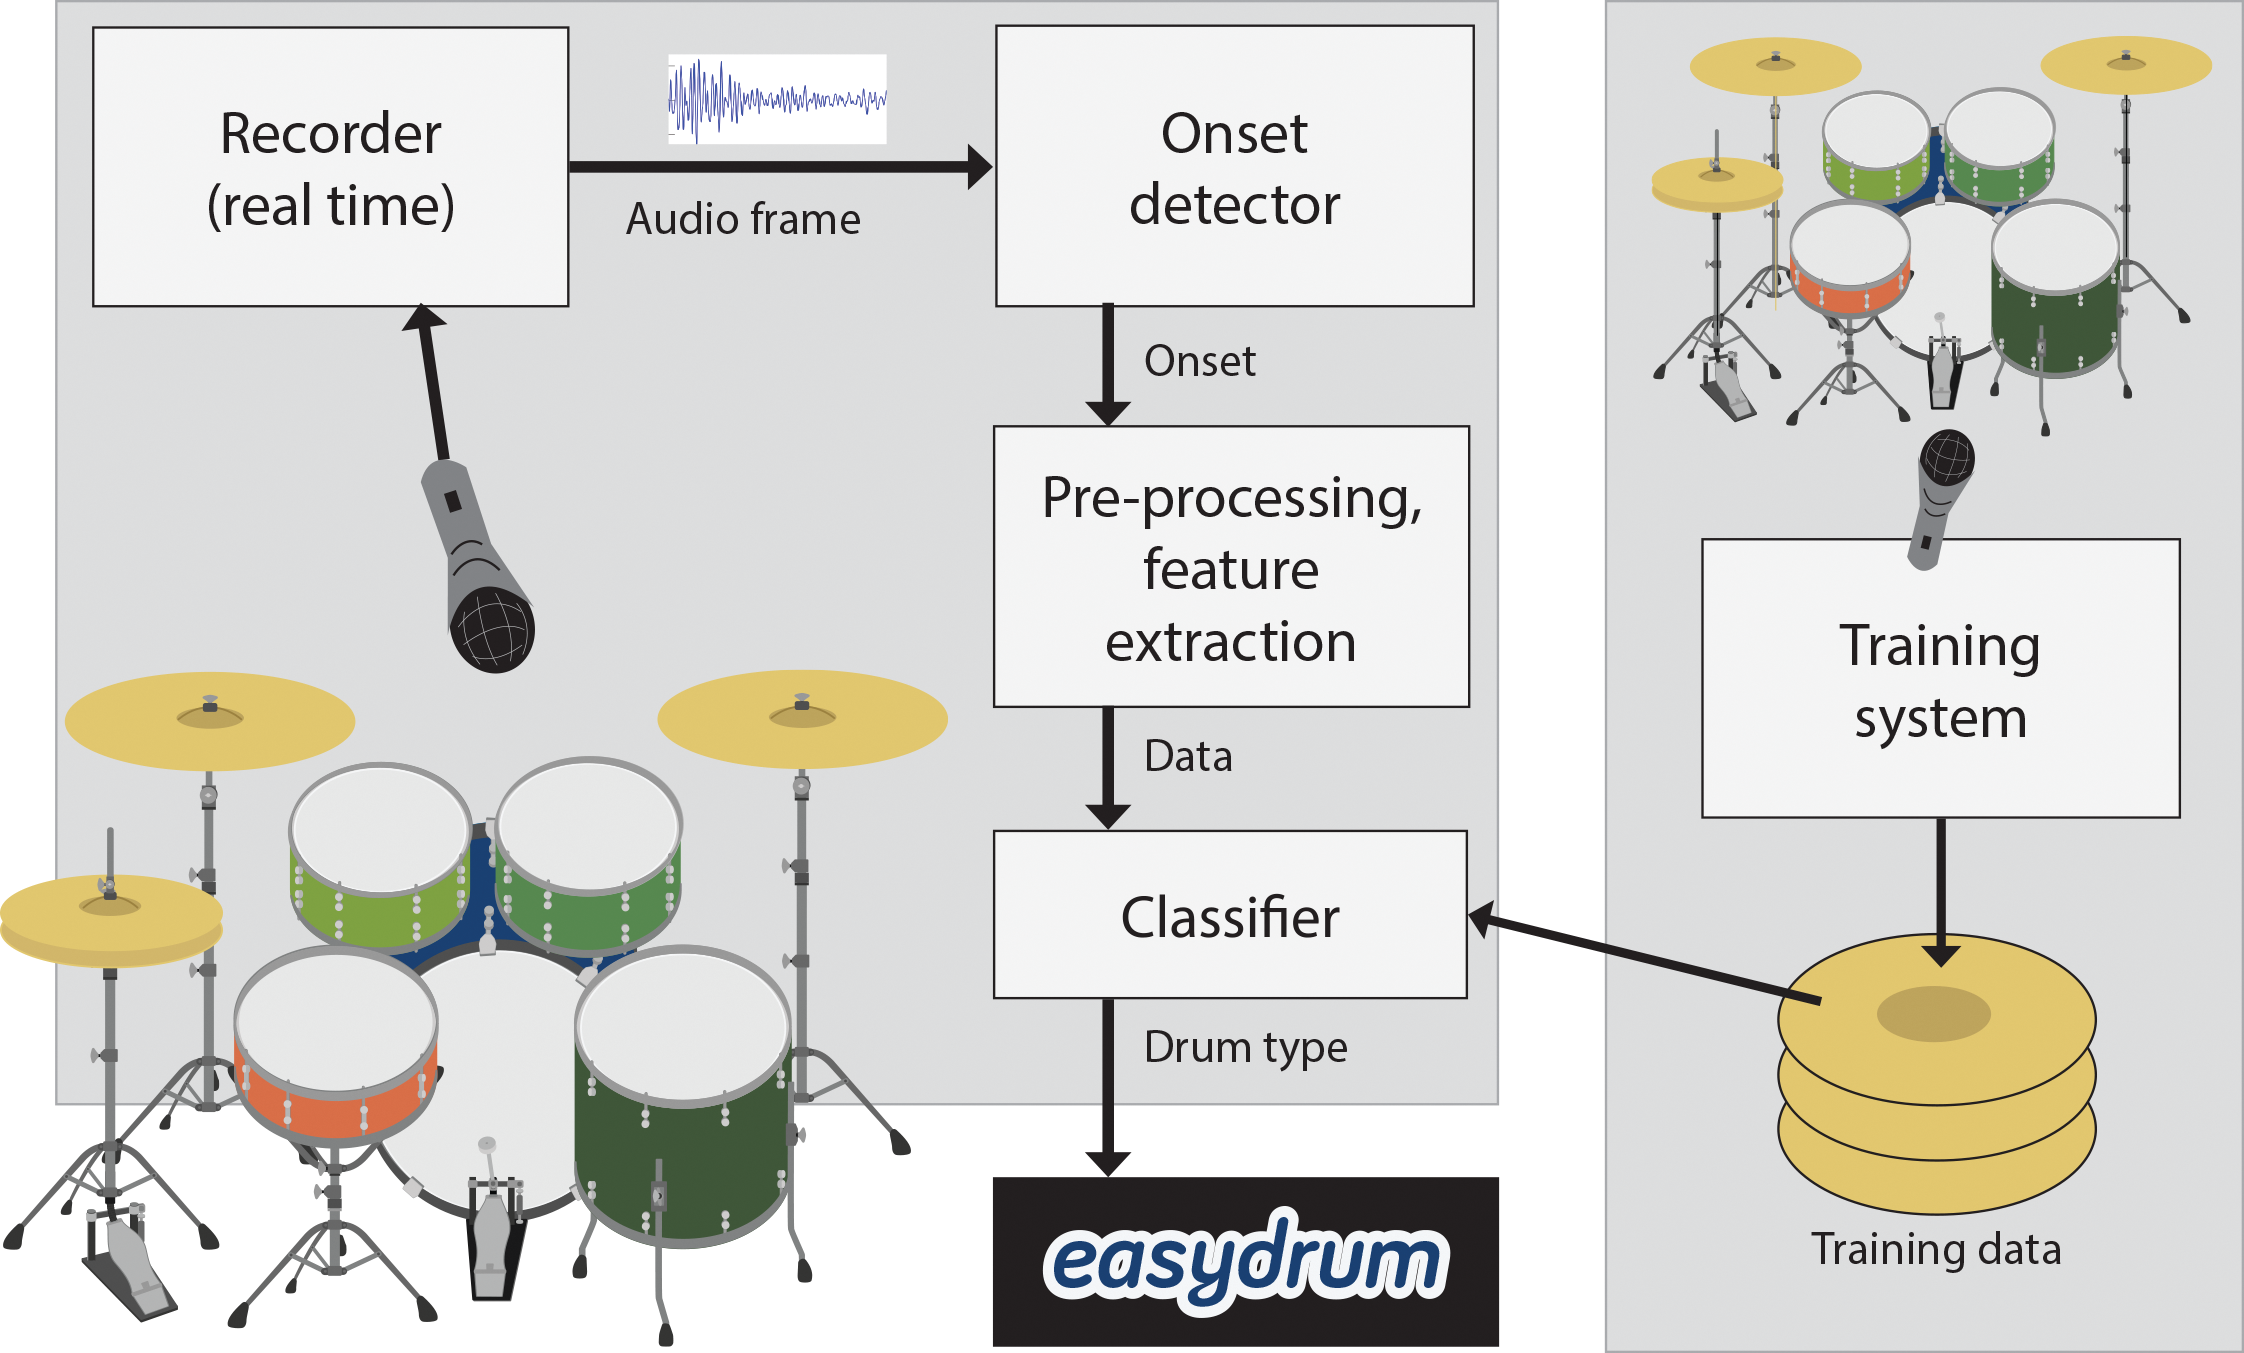
\includegraphics[width=\textwidth]{images/architecture.png}
	\caption{Drum sound analysis software architecture}
	\label{fig:architecture}
\end{figure}

With the help of the training system, the user shall be able to calibrate his drum set to use it with the software. It shall be integrated in the Easydrum drum configurator, which has already been used to configure an electronic drum set.  

The real-time drum analyzer shall be integrated in the Easydrum player. It shall consist of four steps: an audio recorder, an onset detector, a component for pre-precessing and feature extraction and a classifier. The recorder shall record small audio frames and send each of them to the onset detector. The data of each found onset shall be pre-processed for classification. Thereby, required features shall be extracted. The resulting data shall be sent to the classifier, which shall return the determined drum type and send it as an input event to the existing Easydrum player. 

In the following sections, the components required to realize this system are developed with the help of a basic drum set, which is described in section \ref{section:hardware}. An onset detection algorithm is developed that is able to run in real-time in section \ref{section:onsetdetectionmethod}, as well as two different methods for the classification of single drums and cymbals from section \ref{section:classificationSpectrumAnalysis} to section \ref{section:method2}. Furthermore, the second method is tested with simultaneous played strokes in section \ref{section:methodCombined}. The onset detection and classification algorithms are tested with MatLab\textsuperscript{\textregistered}. Finally, this chapter introduces a basic example which uses JavaScript to receive an audio stream via the browser and displays it on an HTML canvas element in section \ref{section:methodJavascript}.

\subsection{Test Drum Set and Hardware} \label{section:hardware}

For the development of the methods in this thesis, a standard drum set, a microphone, an external sound card and a laptop have been used. The used components are displayed in figure \ref{fig:components}.

\begin{SCfigure}[][h]
	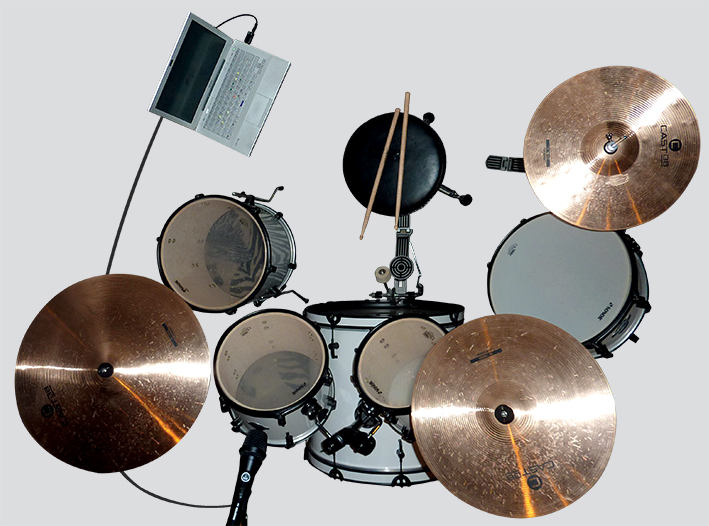
\includegraphics[width=10cm]{images/drumset/drumset_01.jpg}
	\caption{Hardware components 1. Basic drum set (Sonor SFX 11), 2. Maple leaf drumsticks, 3. Dynamic microphone (AKG P3 S), 4. External sound card (LogiLink 7.1), 5. Laptop (Sony VPCSB, 2.7 GHz, 8 GB RAM)}
	\label{fig:components} 
\end{SCfigure}

The used drum set is a basic Sonor SFX 11 drum set that consist of the following components:

\begin{itemize} 
	\item SMF 11 1816 BD WM Bass Drum 18" x 16"
	\item SMF 11 1455 SDW Snare Drum 14" x 5,5"
	\item SMF 11 1008 TT Tom Tom 10" x 8"
	\item SMF 11 1209 TT Tom Tom 12" x 9"
	\item SMF 11 1414 FT Floor Tom 14" x 14"
	\item CB8 Set 1 Cast B8 Cymbals (14" Hi-Hat, 16" Crash, 20" Ride)
	\item Maple wood drum sticks
\end{itemize}

The drum sound is recorded via a dynamic microphone (AKG P3 S) with an audio frequency bandwidth from	40 Hz to 20000 Hz. It is linked to an external USB sound card (LogiLink 7.1) via xlr to 3.5 mm headphone jack. The software runs on an 2.7 GHz Sony VAIO Laptop with 8 GB RAM and the operation system Windows 7.

\subsection{Onset Detection} \label{section:onsetdetectionmethod}

The first step of the system developed in this thesis is to detect the onsets of the drums and cymbals. Therefore, an onset detection algorithm is developed, which is able to run in real-time.

\subsubsection{Test Data}
\begin{figure}[tbp]
	\centering
	\subfloat[Bass drum]{
		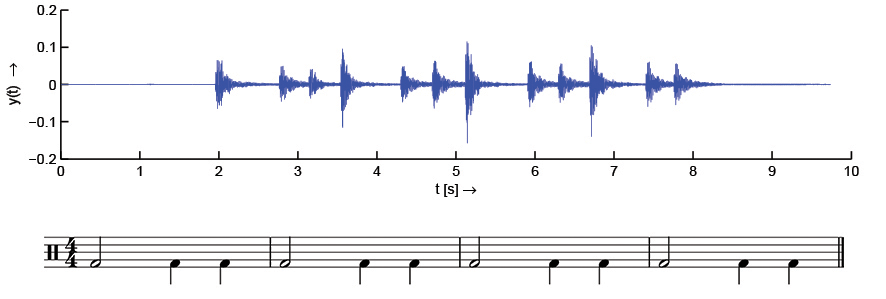
\includegraphics[width=7.3cm]{images/drumsandsheets/drum_bass.png}
	}
	\subfloat[Snare drum 1]{
		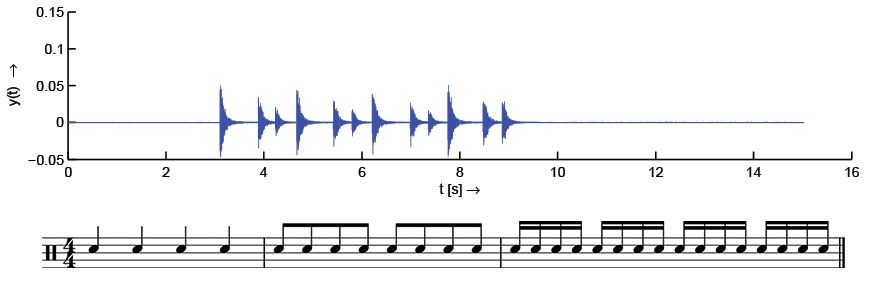
\includegraphics[width=7.3cm]{images/drumsandsheets/drum_snare.png}
	}
	\qquad
	\subfloat[Snare drum 2]{
		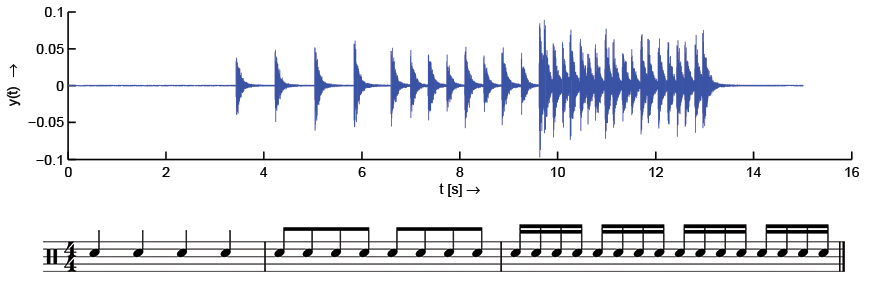
\includegraphics[width=7.3cm]{images/drumsandsheets/drum_snare2.png}
	}
	\subfloat[Tom 1]{
		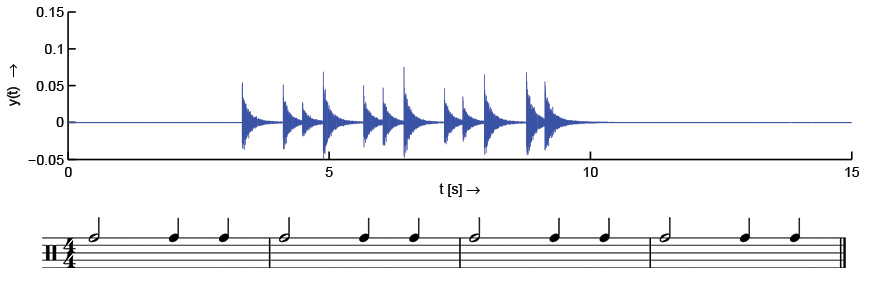
\includegraphics[width=7.3cm]{images/drumsandsheets/drum_tom1.png}
	}
	\qquad
	\subfloat[Tom 2]{
		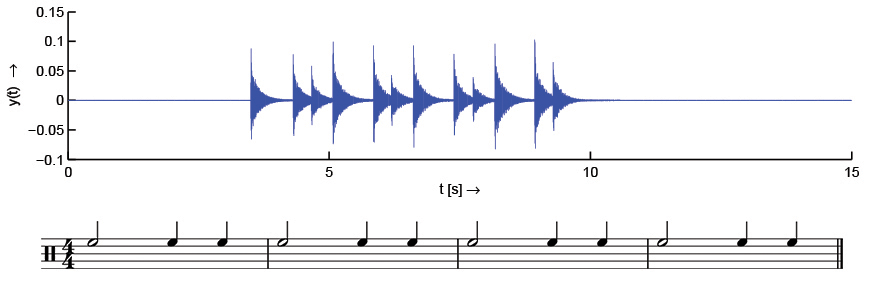
\includegraphics[width=7.3cm]{images/drumsandsheets/drum_tom2.png}
	}
	\subfloat[Tom 3]{
		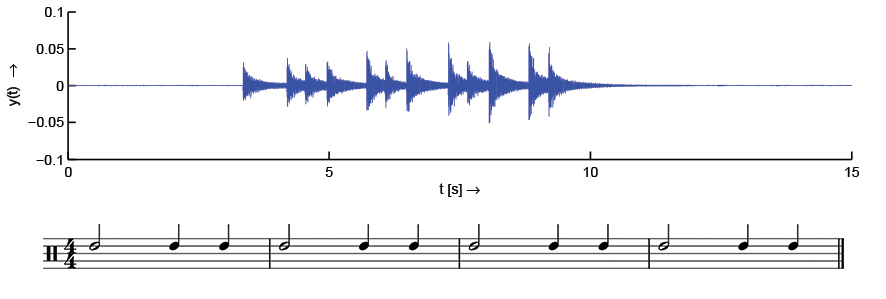
\includegraphics[width=7.3cm]{images/drumsandsheets/drum_tom3.png}
	}
	\caption{Drum loops with single drums.}
	\label{fig:recordings1}
\end{figure}

\begin{figure}[tbp]
	\centering
	\subfloat[Hi-hat closed]{
		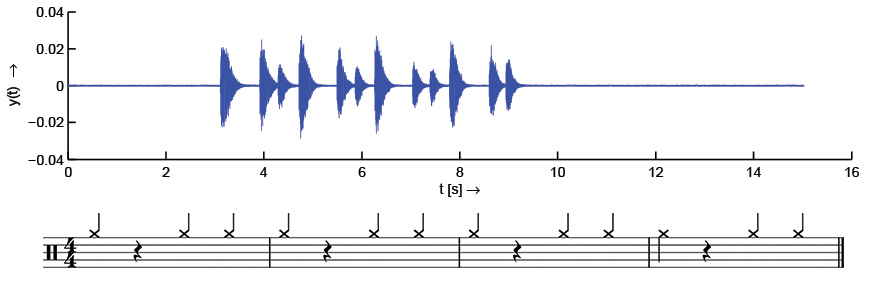
\includegraphics[width=7.3cm]{images/drumsandsheets/drum_hihatclosed.png}
	}
	\subfloat[Hi-hat open]{
		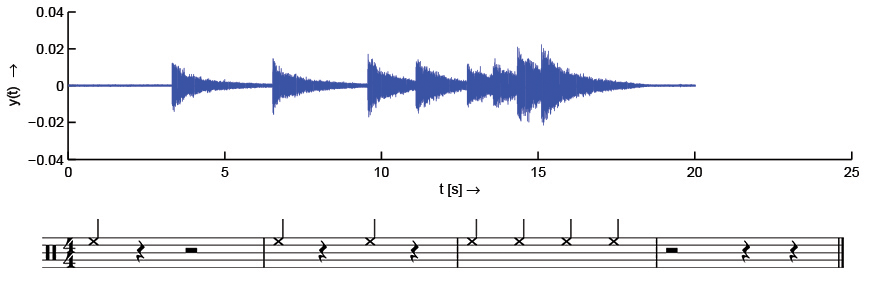
\includegraphics[width=7.3cm]{images/drumsandsheets/drum_hihatopen.png}
	}
	\qquad
	\subfloat[Crash cymbal]{
		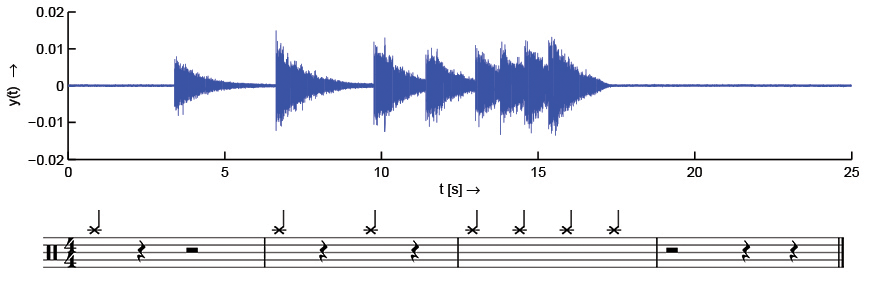
\includegraphics[width=7.3cm]{images/drumsandsheets/drum_crash.png}
	}
	\subfloat[Ride cymbal]{
		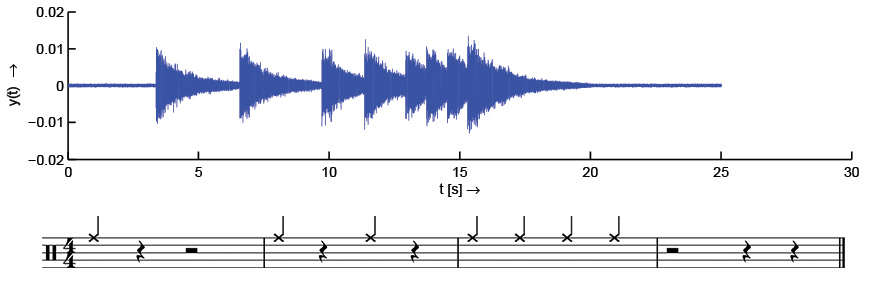
\includegraphics[width=7.3cm]{images/drumsandsheets/drum_ride.png}
	}
	\caption{Drum loops with single cymbals.}
	\label{fig:recordings2}
\end{figure}

\begin{figure}[tbp]
	\centering
	\subfloat[Loop 1]{
		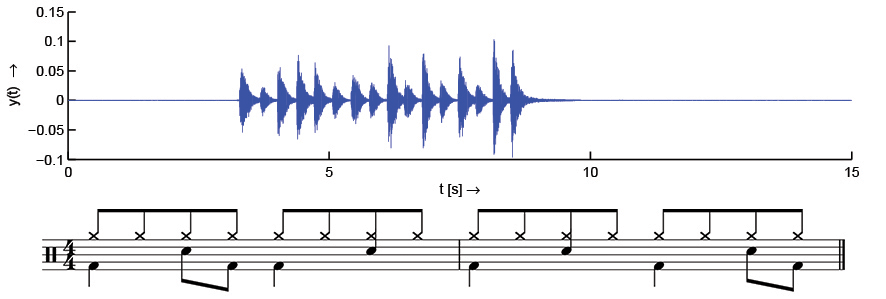
\includegraphics[width=7.3cm]{images/drumsandsheets/loop1.png}
	}
	\subfloat[Loop 2]{
		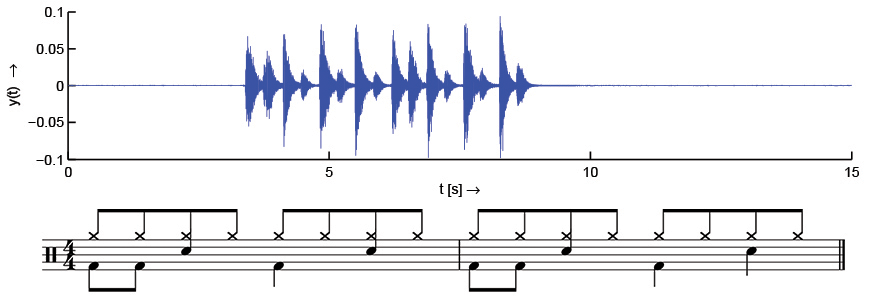
\includegraphics[width=7.3cm]{images/drumsandsheets/loop2.png}
	}
	\qquad
	\subfloat[Loop 3]{
		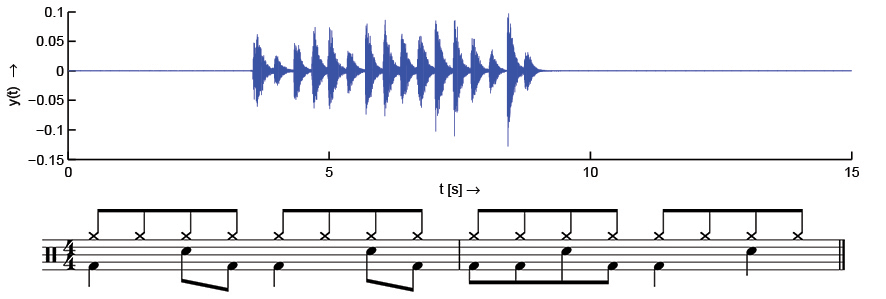
\includegraphics[width=7.3cm]{images/drumsandsheets/loop3.png}
	}
	\subfloat[Loop 4]{
		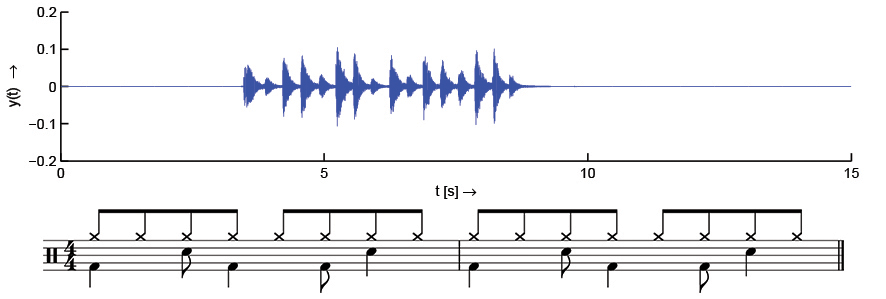
\includegraphics[width=7.3cm]{images/drumsandsheets/loop4.png}
	}
	\caption{Drum loops with bass drum, snare drum and closed hi-hat.}
	\label{fig:recordings3}
\end{figure}

\begin{figure}[tbp]
	\centering
	\subfloat[Fill-in 1 - snare drum, tom 1, tom 2, tom 3]{
		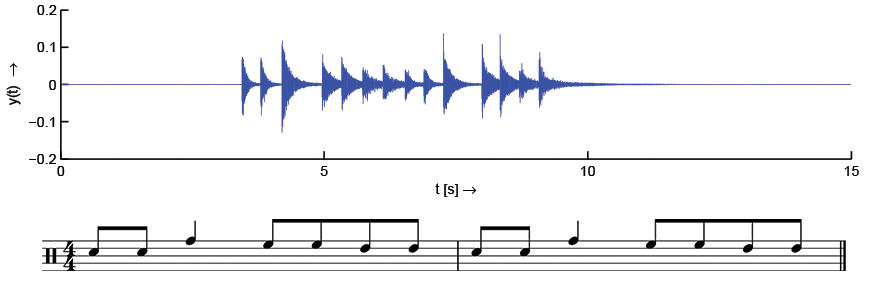
\includegraphics[width=7.3cm]{images/drumsandsheets/fillin1.png}
		\label{fig:fillin1}
	}
	\subfloat[Fill-in 2 - bass drum, snare drum, crash cymbal]{
		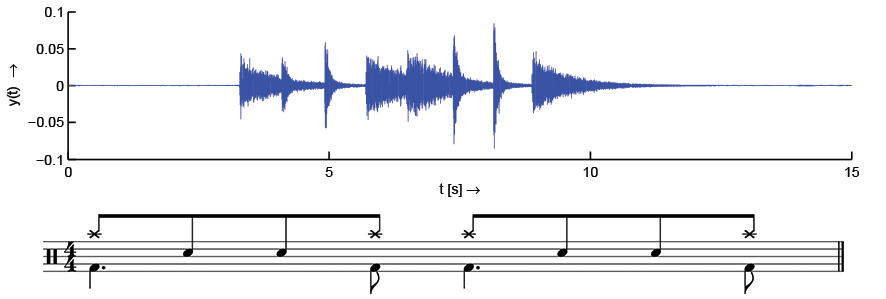
\includegraphics[width=7.3cm]{images/drumsandsheets/fillin2.png}
		\label{fig:fillin2}
	}
	\qquad
	\subfloat[Fill-in 3 - bass drum, snare drum, crash cymbal]{
		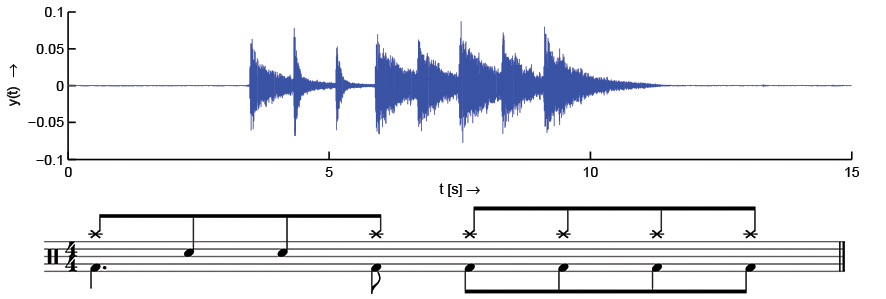
\includegraphics[width=7.3cm]{images/drumsandsheets/fillin3.png}
		\label{fig:fillin3}
	}
	\subfloat[Fill-in 4 - ride cymbal bow and bell]{
		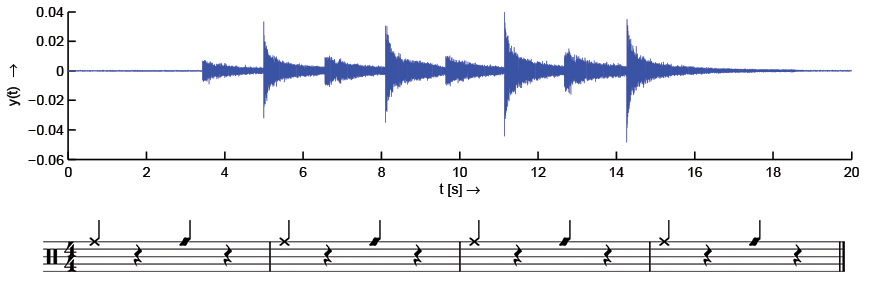
\includegraphics[width=7.3cm]{images/drumsandsheets/fillin4.png}
		\label{fig:fillin4}
	}
	\caption{Fill-ins.}
	\label{fig:recordings4}
\end{figure}

To evaluate the onset detection algorithm developed in the following, there are different short drum loops recorded. They are further used to analyze the waveforms of the different drums and cymbals. Figures \ref{fig:recordings1} to \ref{fig:recordings4} show the audio signals of these recordings with appropriate sheets. The sound files include a recording for each used drum and cymbal in which they are played at different intervals (figure \ref{fig:recordings1} and \ref{fig:recordings2}). For the snare drum there is an additional recording in which it is played faster. Moreover, four drum loops and four fill-ins were recorded. The drum loops (figure \ref{fig:recordings3}) contain common drum rhythms including the bass drum, the snare drum and the closed hi-hat. One of the fill-ins (figure \ref{fig:fillin1}) contains the snare drums and the three tom toms. Two of the fill-ins (figures \ref{fig:fillin2} and \ref{fig:fillin3}) contain the bass drum, the snare drum and the crash cymbal, whereas the crash cymbal is played together with the bass drum. The last fill-in (figure \ref{fig:fillin4}) contains the ride cymbal with rim and bell played alternately.

\subsubsection{Analysis of Drum Recordings}

Before the onset detection algorithm is developed, the recordings are analyzed to figure out which characteristics need to be considered for onset detection. Thereby, it is observed that every stroke on a drum or cymbal produces an explicit rise in amplitude. This rise in energy is followed by the decay of the signal. Hence, the algorithm only needs to be based on the audio wave. There is no need to consider the frequency spectrum. This way, the computing time can be reduced. 

To be able to find the onsets only on the basis of the audio wave, the forms of the different drum strokes need to be regarded. Different drum types vary in their attack and decay time. The decay of all drums shows an inversely proportional form. The cymbals, except the closed hi-hat, decay much slower than the drums. 

The opened hi-hat, the crash cymbal and the ride cymbal show similar waveforms. They decay much slower than the closed hi-hat and the drums. The attack time of these cymbals is nearly zero. The decay can show vibrations. Thus, in the decaying phase of a tone the amplitudes can rise without a new stroke. The crash cymbal shows most vibrations, the opened hi-hat the least. The closed hi-hat can also show vibrations, but it decays much faster. In contrast to the other cymbals, it has a higher attack time. This means that its amplitude rises for a short time period after the onset. This phenomenon can also be observed for the bass drum. It even has a longer attack time than the hi-hat. Furthermore, there are more vibrations, whilst the decay time is similar. The remaining drums show no significant attack time or vibrations. While the tom toms decay slower than the bass drum, the snare drum shows the shortest decay time of all considered drums and cymbals. It decays slightly shorter than the hi-hat and bass drum. 

Hence, for the onset detector it is significant to support different decay times, and not to detect vibrations and rising amplitudes during the attack as onsets.

\newpage
\subsubsection{Method}

The developed onset detection algorithm is based on the algorithm in \autocite{Schloss:1985}, which is described in section \ref{section:OnsetDetectionSchloss}. Schloss uses a fast and simple algorithm which only considers the amplitude envelope of the audio wave. As a stroke on a drum always produces an increase in the amplitude envelope, this is a good method to achieve a short computing time. Moreover, Schloss considers subsequent frames of an audio file to detect the onsets. Thus, the algorithm described in \autocite{Schloss:1985} provides the required features to run in real-time.

Hence, based on the method of Schloss, the algorithm developed in this thesis scans subsequent recorded frames for sudden rises in the amplitude of the audio wave. Therefore, the actual frame is compared to the mean of a given number of preceding frames. The algorithm is able to run in real-time. It is implemented as a MatLab\textsuperscript{\textregistered} class called \textit{DetectOnset}. An UML diagram of the class is shown in figure \ref{fig:onsetDetectorUML}.

\begin{figure}[htb]
	\centering
	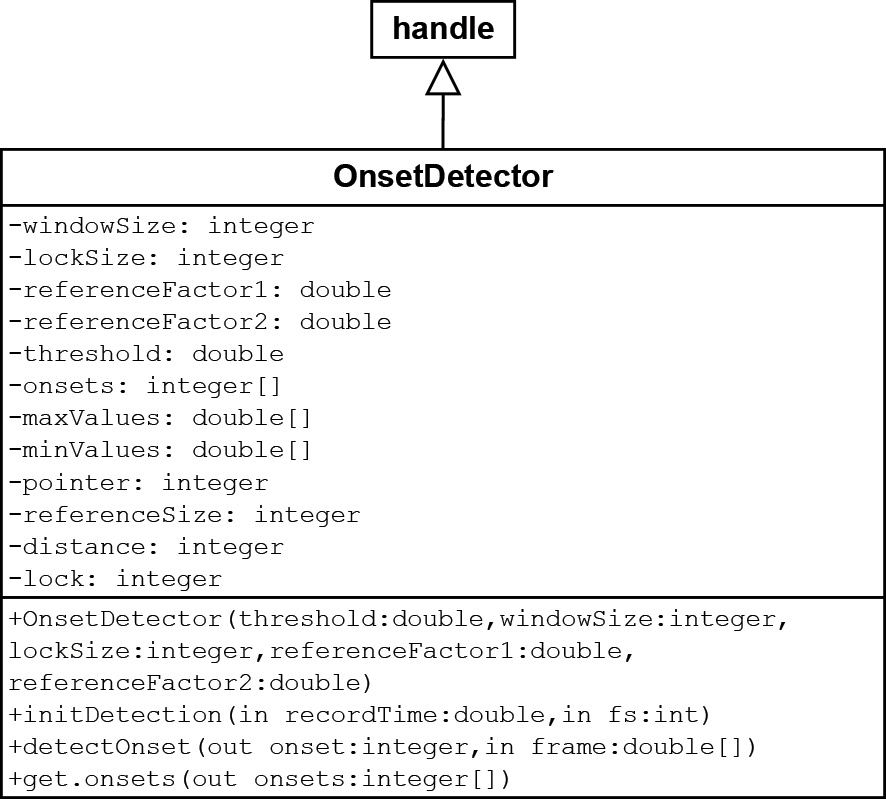
\includegraphics[width=7.5cm]{images/UML/onsetDetectorUML.png}
	\caption{UML diagram of the onset detector}
	\label{fig:onsetDetectorUML}
\end{figure}

The class has the properties \lstinline{threshold} (data type double), \lstinline{windowSize} (data type integer), \lstinline{lockSize} (data type integer), \lstinline{referenceFactor1} (data type double), \lstinline{referenceFactor2} (data type double), \lstinline{onsets} (vector of data type integer), \lstinline{maxValues} (vector of data type double), \lstinline{minValues} (vector of data type double), \lstinline{pointer} (data type integer), \lstinline{referenceSize} (data type integer), \lstinline{distance} (data type integer) and \lstinline{lock} (data type integer).

\begin{sloppypar}
The property values for \lstinline{threshold}, \lstinline{windowSize},  \lstinline{lockSize}, \lstinline{referenceFactor1} and \lstinline{referenceFactor2} are set by the constructor. Whereas the threshold always needs to be specified, there are default values for the remaining parameters. If they are not passed, the values are set to \lstinline{windowSize=512}, \lstinline{lockSize=8}, \lstinline{referenceFactor1=1} and \lstinline{referenceFactor2=0.5}. The parameter \lstinline{referenceFactor1} should contain a value greater than one and \lstinline{referenceFactor2} a value between zero and one.
\end{sloppypar}

The parameter \lstinline{threshold} defines the minimum amplitude that can be declared as an onset. With the help of this parameter the algorithm defining the noise of the recording or low background sounds as onsets is avoided. For testing method developed in this thesis, the threshold is defined by analyzing a frame that only contains noise. The maximum value of this frame multiplied with the factor five is chosen as the threshold value. Thus, an onset must have the minimum amplitude of five times the maximum noise amplitude.

The parameter \lstinline{windowSize} defines the size of the frames in which the audio file is segmented. 

The parameter \lstinline{lockSize} defines the size of the lock, which is set after every onset. This lock prohibits to find two onsets in an interval of a given number of frames after an onset. It is needed because the amplitude rises a certain time after the onset. Furthermore, especially the amplitude of a cymbal can be very unstable. Thus, in this time interval there should be no more onset detected because it would be produced by the same stroke. 

The vectors \lstinline{minValues} and \lstinline{maxValues} are used to save the minimum and maximum amplitudes of each frame. 

The property \lstinline{pointer} saves the number of recently processed frames during the runtime of the current onset detection process. Thus, it points to the index of the last added value in the vectors \lstinline{minValues} and \lstinline{maxValues}.

The properties \lstinline{referenceSize}, \lstinline{distance} and \lstinline{lock} store non-static values, which are changing during the runtime of the algorithm. 

The property \lstinline{distance} saves the number of frames from the currently considered frame to the frame with the last found onset. 

The property \lstinline{referenceSize} defines the number of preceding frames considered when analyzing a frame for an onset. It is used to calculate the values of \lstinline{minReference} and \lstinline{maxReference}, which save two thresholds. To be declared as an onset, the frame must contain an amplitude smaller than \lstinline{minReference} and an amplitude greater than \lstinline{maxReference}. The maximum amplitude is calculated by the mean of all maxima in the preceding frames multiplied with the value of \lstinline{referenceFactor1}, which is transferred to the onset detector as a parameter. The minimum amplitude is calculated in the same way, with the difference that the minimum values are used. Thereby, \lstinline{minReference} may not be greater than \lstinline{-threshold} and \lstinline{maxReference} may not be smaller than \lstinline{threshold}. Listing \ref{lst:onset1} shows the appropriate MatLab\textsuperscript{\textregistered} code.

%[\label{listing:onset1}]
\begin{lstlisting}[caption={Calculation of minReference and maxReference},label={lst:onset1}]
minReference= ...
		mean(obj.minValues(obj.pointer-obj.referenceSize-1:obj.pointer-1)) ...
		*obj.referenceFactor1;
maxReference= ...
		mean(obj.maxValues(obj.pointer-obj.referenceSize-1:obj.pointer-1)) ...
		*obj.referenceFactor1;

if (minReference > obj.threshold) minReference=-obj.threshold; end
if (maxReference < obj.threshold) maxReference=obj.threshold; end  
\end{lstlisting}

%- Die Variable lock definiert eine Sperre. Ist die Sperre aktiviert kann kein Onset vorliegen. Nachdem ein Onset gefunden wurde wird lock gleich dem Parameter lock_size gesetzt. Nach jedem Frame wird lock um eins vermindert. Nur wenn lock null ist, kann ein Onset gefunden werden.
The property \lstinline{lock} saves the status of the lock. It is set to the size of the parameter \lstinline{lockSize} after an onset is detected and otherwise downsized by one. The minimum value of \lstinline{lock} is zero. If the value is greater than zero, the lock is activated and no onset can be found. Thus, an onset can only be detected if \lstinline{lock} is equal to zero.   

To calculate the value for \lstinline{referenceSize}, the parameter \lstinline{referenceFactor2} is needed. It defines the percentage of frames from the currently considered frame to the frame with the last onset. Within the MatLab\textsuperscript{\textregistered} function the value is calculated by \lstinline{referenceSize=ceil(distance*referenceFactor2)}. Hence, the higher the distance to the last onset, the higher the value for \lstinline{referenceSize}. After an onset has been found, \lstinline{referenceSize} is reset to one.

%Die reference_size wird größer, je weiter der letzte Onset zurückliegt. Es werden nur Frames betrachtet, die nach dem letzten Onset liegen. Je weiter dieser zurück liegt, desto mehr Frames liegen also zwischen letztem Onset und gerade analysiertem Frame, desto mehr Frames können betrachtet werden, um den Mittelwert zu berechnen. Da die Amplitude nach einem Onset langsam abnimmt, muss auch der Referenzwert für einen neuen Onset abnehmen. Der als Referenzwert berechnete Mittelwert darf also nicht zu groß werden, da dadurch unter Umständen ein Onset mit geringerer Amplitude als der vorangehende nicht entdeckt wird. Dies wird dadurch vermieden, dass bei der Berechnung von min_reference/max_reference nicht alle Frames bis zum letzten Onset genutzt werden. Die Anzahl der Frames, die betrachtet werden wird durch ceil(distance/reference_denominator) berechnet.
The variation of the property \lstinline{referenceSize} is a decisive part of the algorithm. It is based on the fact that the amplitude decays inversely proportional after an onset. Thereby, some stroke types decay faster than others. Hence, the higher the distance to the last onset, the slower the sound decays and the smaller the amplitude difference when comparing the actual frame with the mean of the preceding ones. By rising the number of frames for comparison, the calculated mean values do also rise. Thus, the amplitude rise has to be greater than it had to be if it would be compared with less frames. This way, the detection of small rises in amplitude, which are caused by vibrations, as false onsets is avoided. Contrariwise, the comparison may also not include too many frames because if the mean value is too high, onsets with lower amplitudes than the preceding one would not be detected.

The vector \lstinline{onsets} saves the positions of all found onsets. It can be read with the help of the  getter function \lstinline{onsets=get.onsets(obj)}.

The function \lstinline{start} needs to be called to initialize a new onset detection process. It is used both before the start of the first onset detection process and to reset the onset detector to begin the detection for a new recording. The function receives the parameters \lstinline{recordTime} and \lstinline{fs}. 

The parameter \lstinline{recordTime} is the period of time in seconds that the onset detection process will be running. In the final system this time will be the duration of the played exercise. If an audio file is scanned it is the duration of the record. The parameter \lstinline{fs} is the sampling rate of the audio input in frames per second. The parameters are needed here to predefine the length of the vectors \lstinline{minValues} and \lstinline{maxValues} and thus to allocate the appropriate memory. It is calculated by \lstinline{ceil(recordTime/(obj.windowSize/fs))}. Further on, the \lstinline{start} function sets the values for the properties \lstinline{pointer}, \lstinline{distance} and \lstinline{lock} to zero and the value for \lstinline{referenceSize} to one. 

After the onset detector is started, the function \lstinline{detectOnset}, which is the essential part of the onset detection algorithm, has to be called for every incoming frame. It receives the audio data as input argument, and if an onset is found, it returns the position of the sample containing the onset. The position is calculated by \lstinline{obj.pointer*obj.windowSize+maxIdx}, whereas \lstinline{maxIdx} defines the index of the actual frames maximum amplitude. If there is no onset found the function returns zero.

The function \lstinline{detectOnset} scans each frame for an onset as follows:

\begin{enumerate}
	\item The variable \lstinline{onset} is defined and set to zero.
	\item \lstinline{pointer} is increased by one.
	\item The minimum and maximum amplitudes of the particular frame are identified and stored in the arrays \lstinline{minValues} and \lstinline{maxValues}. The index of the maximum amplitude is saved as the variable \lstinline{maxIdx}.
	\item If the actual value of the property \lstinline{pointer} is greater than the value of \lstinline{referenceSize+1}, the function proceeds with the next step, otherwise the function returns.
	\item The variables \lstinline{minReference} and \lstinline{maxReference} are calculated as shown in listing \ref{lst:onset1}.
	\item  If the minimum value of the considered frame is smaller than \lstinline{minReference}, the maximum value higher than \lstinline{maxReference} and there is no lock set, the function proceeds with step 6a, otherwise it proceeds with step 6b.
	\begin{enumerate}
		\item The actual maximum position is declared as an onset. The onsets position is calculated by \lstinline{obj.pointer*obj.windowSize+maxIdx}. It is saved in the variable \lstinline{onset} and appended to the vector \lstinline{onsets}. Further on, the property \lstinline{referenceSize} is reset to one, \lstinline{distance} to zero and \lstinline{lock} to \lstinline{lockSize}. It is proceeded with step 7.
		
		\item The property \lstinline{distance} is set to one and the property \lstinline{referenceSize} is calculated by \lstinline{ceil(obj.distance*obj.referenceFactor2)}. It is proceeded with step 7.
	\end{enumerate}
	\item If the property \lstinline{lock} is	greater than zero, it is decreased by one.				
\end{enumerate}

The entire \lstinline{detectOnset} function is displayed in listing \ref{lst:detectOnset}.

\begin{lstlisting}[caption={detectOnset},label={lst:detectOnset}]
function onset=detectOnset(obj,frame)
	onset=0;
	obj.pointer=obj.pointer+1;
  [maxValue,maxIdx]=max(frame);
	obj.minValues(obj.pointer)=min(frame);
	obj.maxValues(obj.pointer)=maxValue;
	
	if obj.pointer>obj.referenceSize+1 
		minReference=  ...
				mean(obj.minValues(obj.pointer-obj.referenceSize-1:obj.pointer-1)  ...
				*obj.referenceFactor1;
		maxReference=  ...
				mean(obj.maxValues(obj.pointer-obj.referenceSize-1:obj.pointer-1))  ...
				*obj.referenceFactor1;

		if (minReference > obj.threshold) minReference = -obj.threshold; end
		if (maxReference < obj.threshold) maxReference = obj.threshold; end  

		if (obj.minValues(obj.pointer) < minReference  ...
		&& obj.maxValues(obj.pointer) > maxReference && obj.lock==0) 
			onset=obj.pointer*obj.windowSize+maxIdx; 
			obj.onsets=[obj.onsets,onset];
			obj.referenceSize=1;
			obj.distance=0;
			obj.lock=obj.lockSize;
		else
			obj.distance=obj.distance+1;
			obj.referenceSize=ceil(obj.distance*obj.referenceFactor2);
		end
		if obj.lock > 0
			obj.lock=obj.lock-1;
		end            
	end	
end
\end{lstlisting}


\subsubsection{Tests}

To test the algorithm, it is applied to the previously recorded sound files. These recordings contain a total of 226 onsets.

A MatLab function reads in the files and splits them into frames with the size of a given value for the parameter \lstinline{windowSize}. For each record, an instance of the class \lstinline{OnsetDetector} is created and its \lstinline{start} function is called. Subsequent, the appropriate frames are sent to the \lstinline{onsetDetection} function. The resulting array of onsets for each record is drawn to a figure. To improve the hit-rate, the parameters \lstinline{windowSize}, \lstinline{lockSize}, \lstinline{referenceFactor1} and \lstinline{referenceFactor2} are varied. 

It is important to choose a convenient window size to enable the algorithm to run in real-time. If the frame size is too small, the algorithm needs too long to perform during the runtime. If it is too large, the resolution is too small and a detected onset is returned too late. Moreover, onsets can be missed because two onsets are located within the same frame. It also needs to be considered that the number of onsets can rise when choosing a small frame size because vibrations are split to several frames and thus declared as onsets. The best results have been gained with a frame size of 512 samples, which equals 11.6 ms. The lock size is set to 8. Thus, there is a lock for a total of 4096 ($8*512$) samples. This equals 92 ms during which no further onset can be detected. The value for \lstinline{referenceFactor1} is found to be effective between 1.4 and 1.6 in combination with \lstinline{referenceFactor2} between 0.4 and 0.5. 

The best results have been gained by using the values 1.52 for \lstinline{referenceFactor1} and 0.4 for \lstinline{referenceFactor2}. There is one onset missing and one false positive onset. The results are shown in figure \ref{fig:onsetTest1}. The missing onset is a stroke on the snare drum in figure \ref{fig:onsetTest1_1}. At this part of the record the snare drum is played fast. The stroke is to close to the preceding one and the minimum amplitude of the stroke is much lower, but the used factors \lstinline{referenceFactor1=1.52} and \lstinline{referenceFactor2=0.4} produce a lower value for \lstinline{minReference}, here. Hence, the stroke cannot be detected. The false positive is a stroke on the crash cymbal, the cymbal which creates the strongest vibrations. At the point where the false onset is detected the amplitude rises even higher than at the onset itself. Thus, the calculated values for \lstinline{minReference} are too low and for \lstinline{maxReference} too high, which causes the false detection of the onset. The stroke is placed in figure \ref{fig:onsetTest1_2}.

\begin{sloppypar}
Figure \ref{fig:onsetTest2} shows the results with the use of the factors \lstinline{referenceFactor1=1.45} and \lstinline{referenceFactor2=0.45}. With these lower factors the detection of all onsets can be achieved, but the number of false detected onsets rises to five. The results are shown in figure \ref{fig:onsetTest2}. Contrarily, trying to avoid false onsets leads to a rise in the number of missing ones. To test this, the factors are set to \lstinline{referenceFactor1=1.6} and \lstinline{referenceFactor2=0.5}. The results are displayed in figure \ref{fig:onsetTest3}. There are no false onsets, but four of the onsets are not detected by the algorithm.
\end{sloppypar}

\begin{figure}[bp]
	\centering
	\subfloat[Bass drum]{
		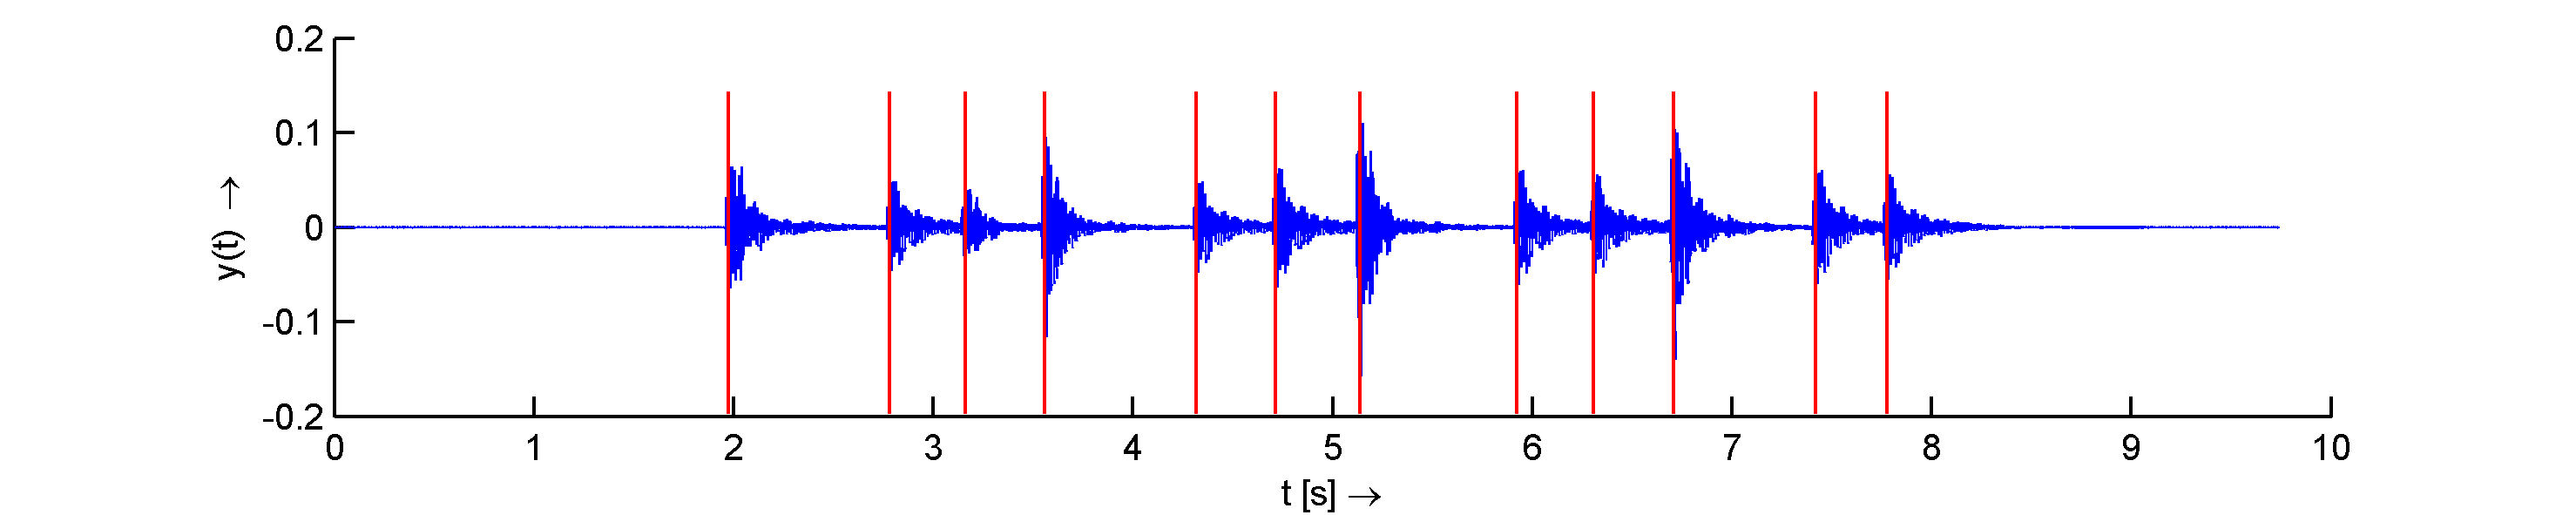
\includegraphics[width=7cm]{images/onsettest/1/drum_bass.png}
	}
	\subfloat[Snare drum 1]{
		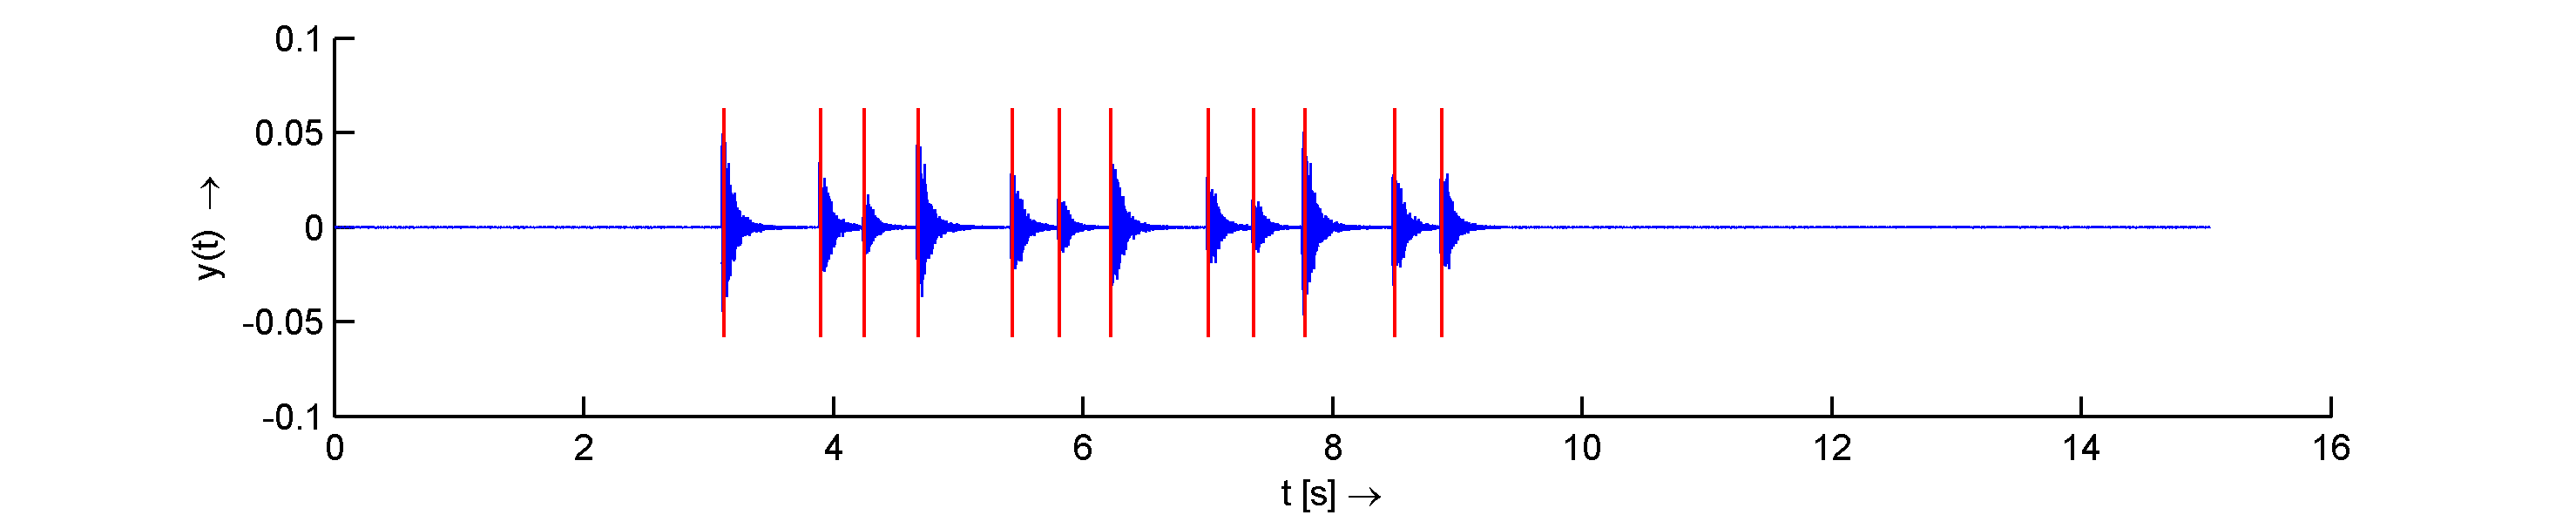
\includegraphics[width=7cm]{images/onsettest/1/drum_snare.png}
	}
	\qquad
	\subfloat[Snare drum 2]{
		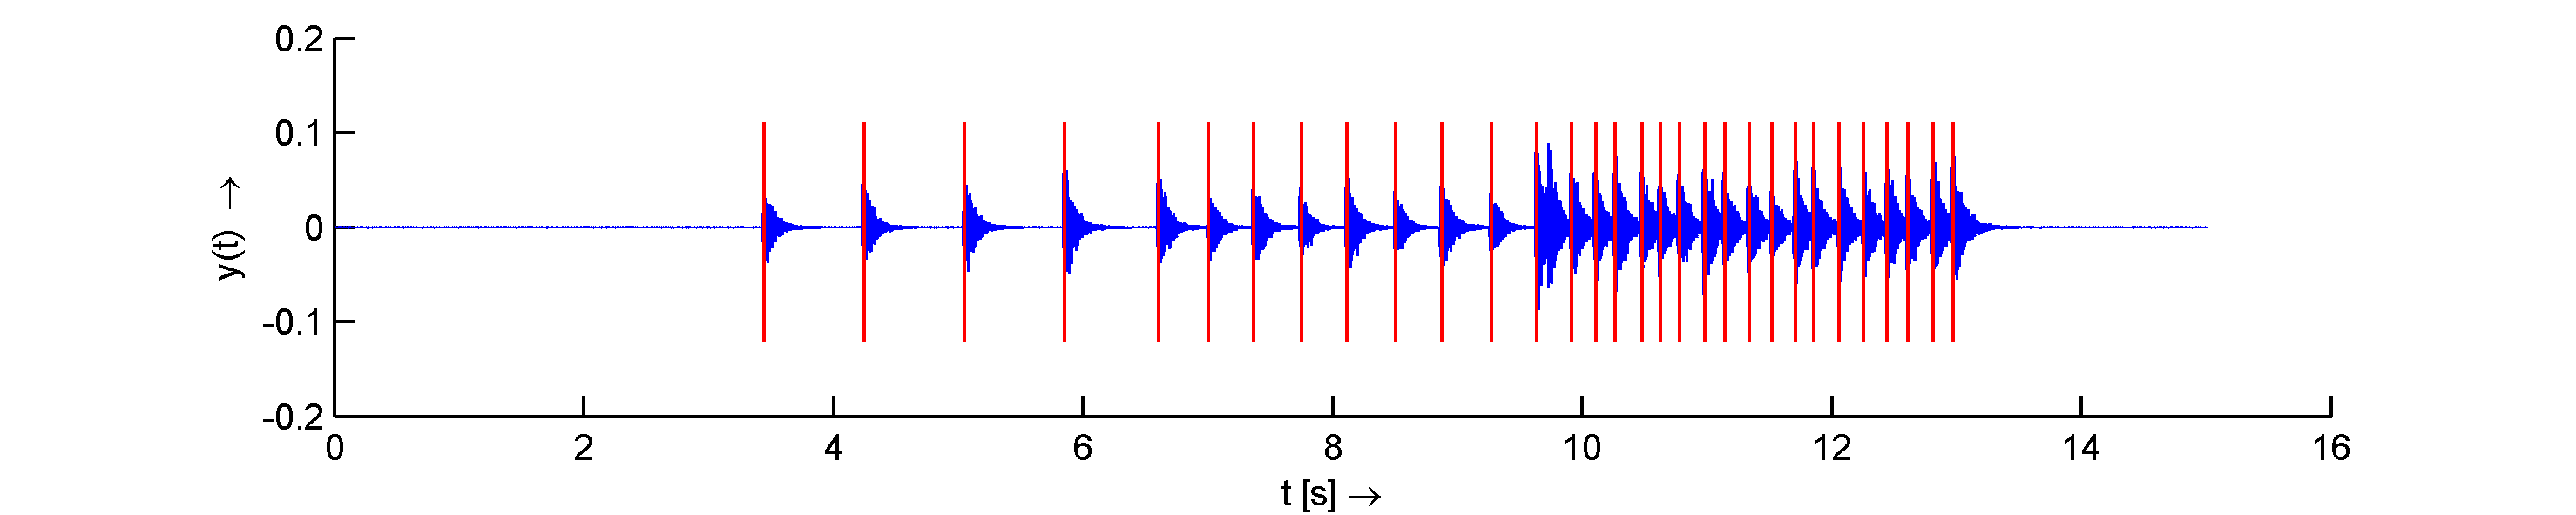
\includegraphics[width=7cm]{images/onsettest/1/drum_snare2.png}
	\label{fig:onsetTest1_2}
	}
	\subfloat[Tom 1]{
		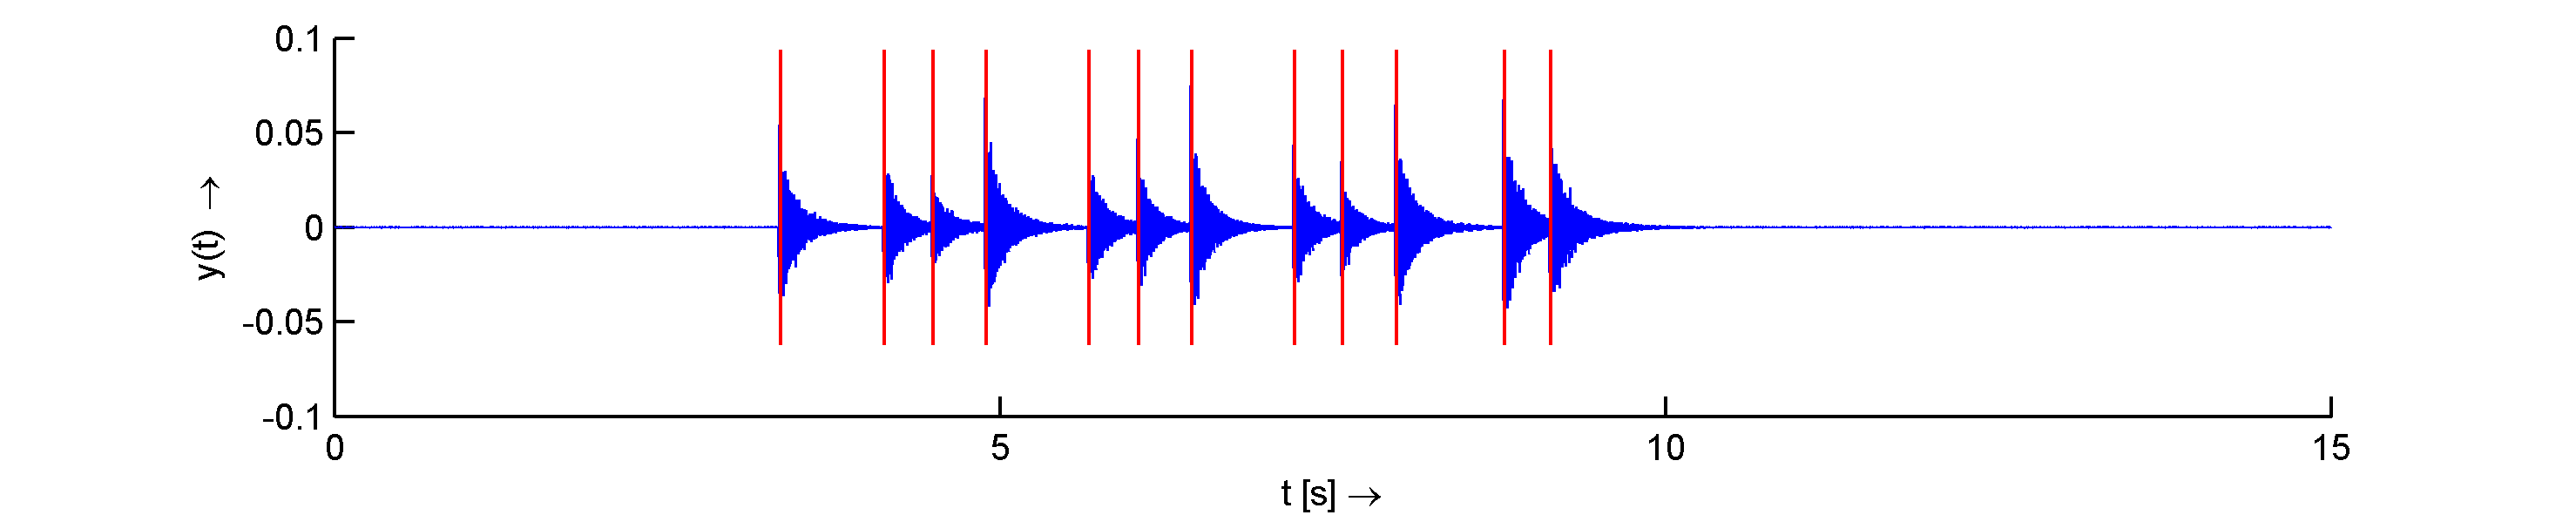
\includegraphics[width=7cm]{images/onsettest/1/drum_tom1.png}
	}
	\qquad
	\subfloat[Tom 2]{
		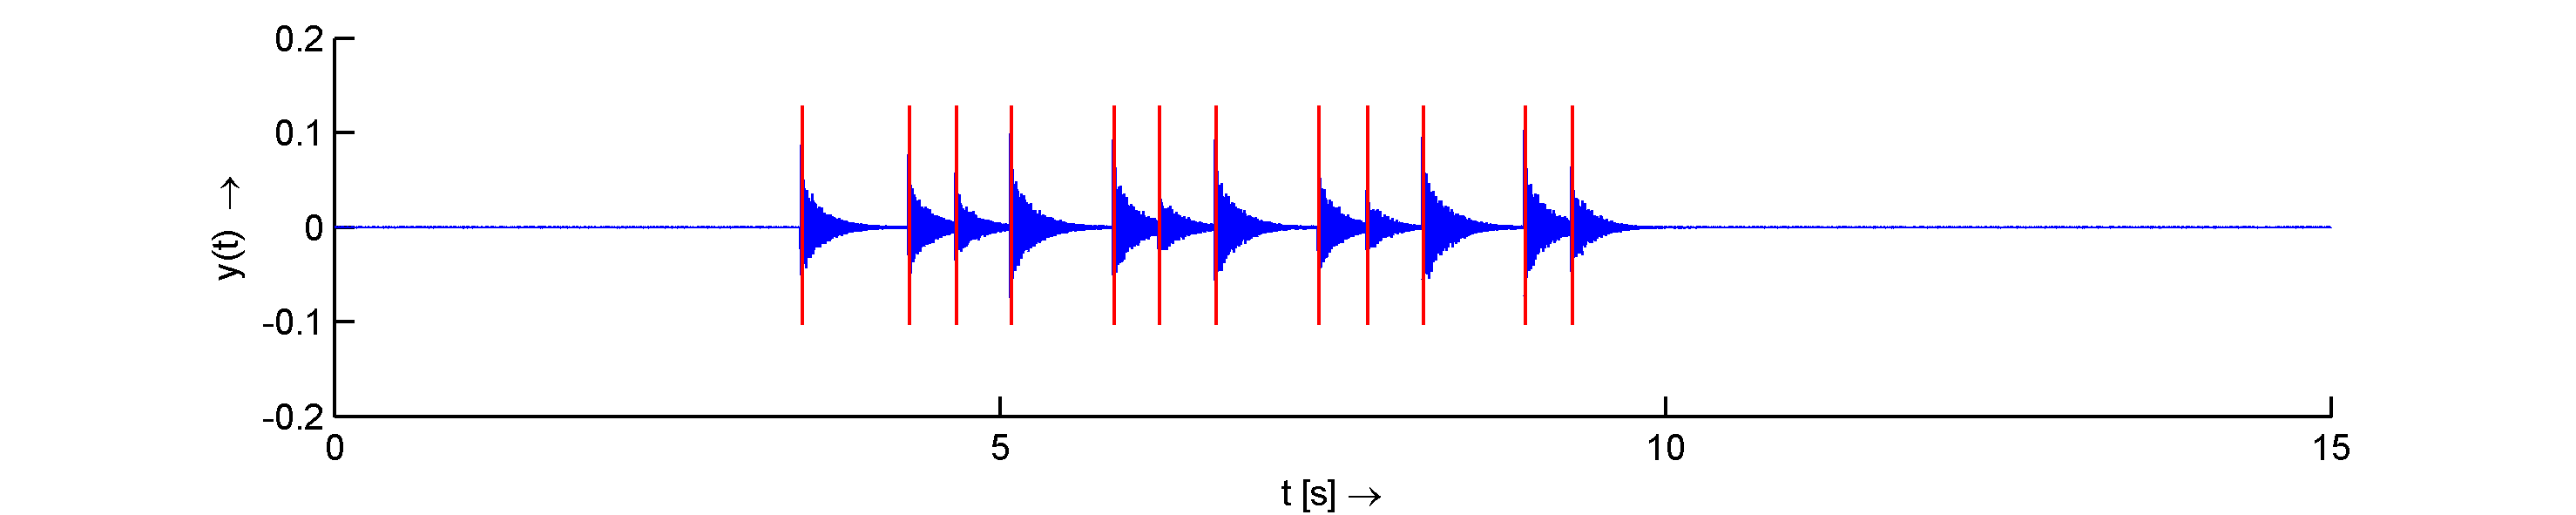
\includegraphics[width=7cm]{images/onsettest/1/drum_tom2.png}
	}
	\subfloat[Tom 3]{
		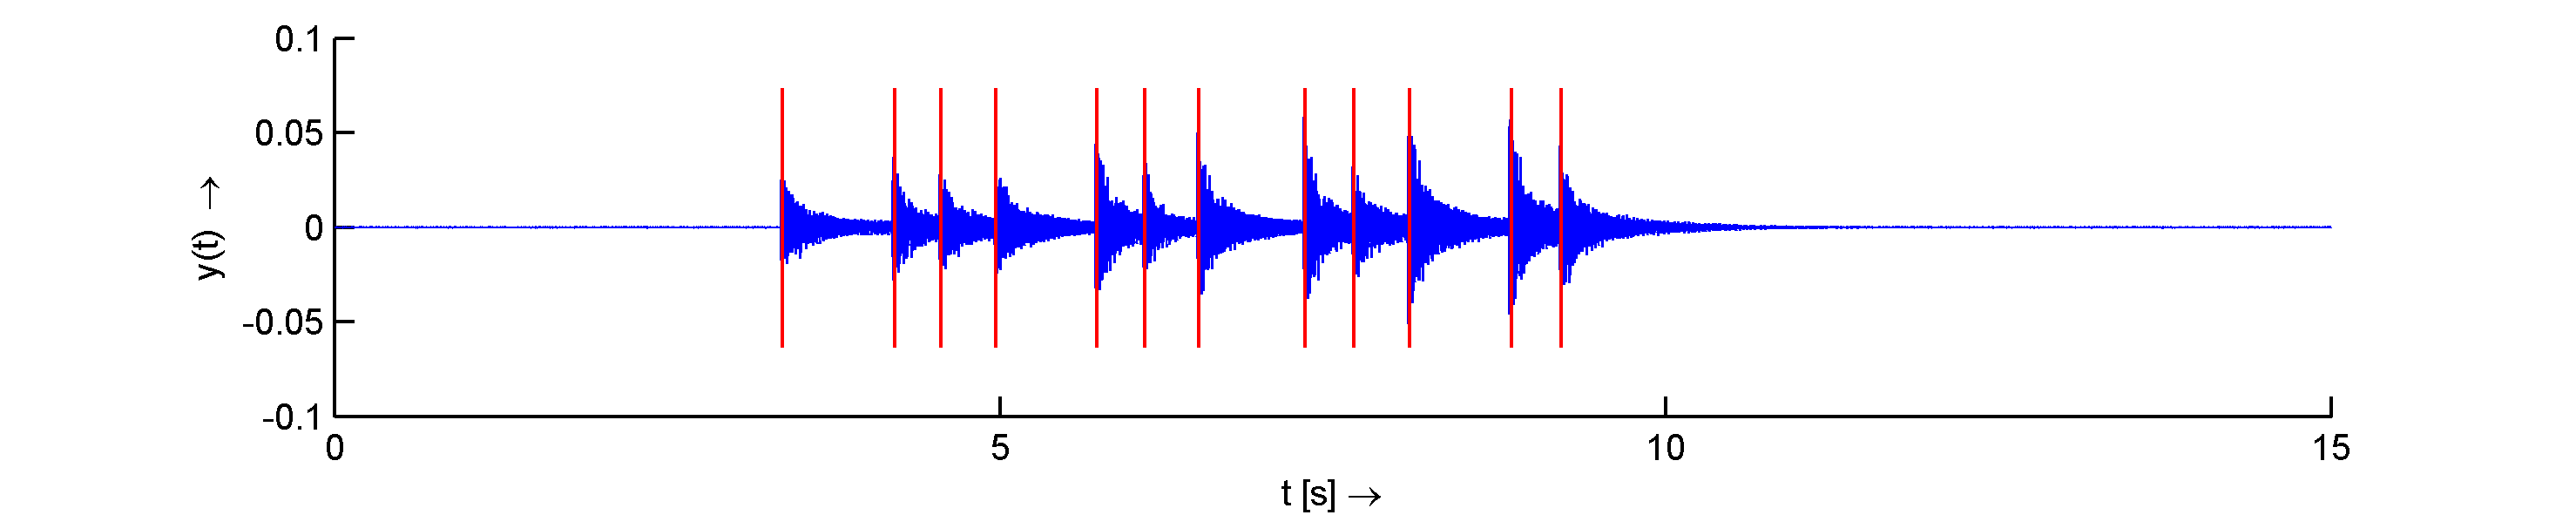
\includegraphics[width=7cm]{images/onsettest/1/drum_tom3.png}
	}
	\qquad
	\subfloat[Hi-hat closed]{
		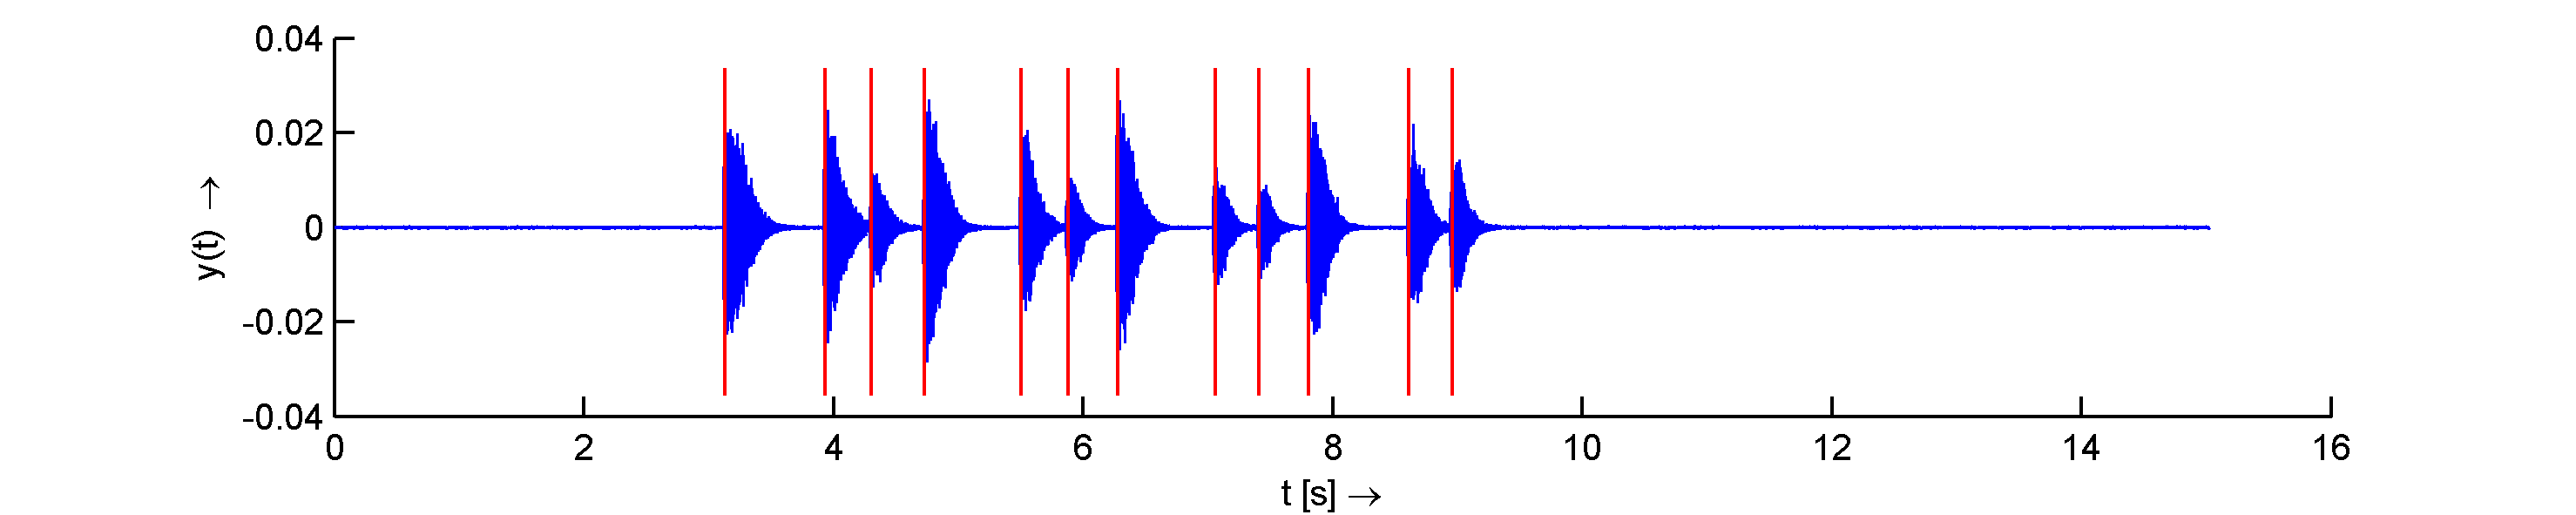
\includegraphics[width=7cm]{images/onsettest/1/drum_hihatclosed.png}
	}
	\subfloat[Hi-hat open]{
		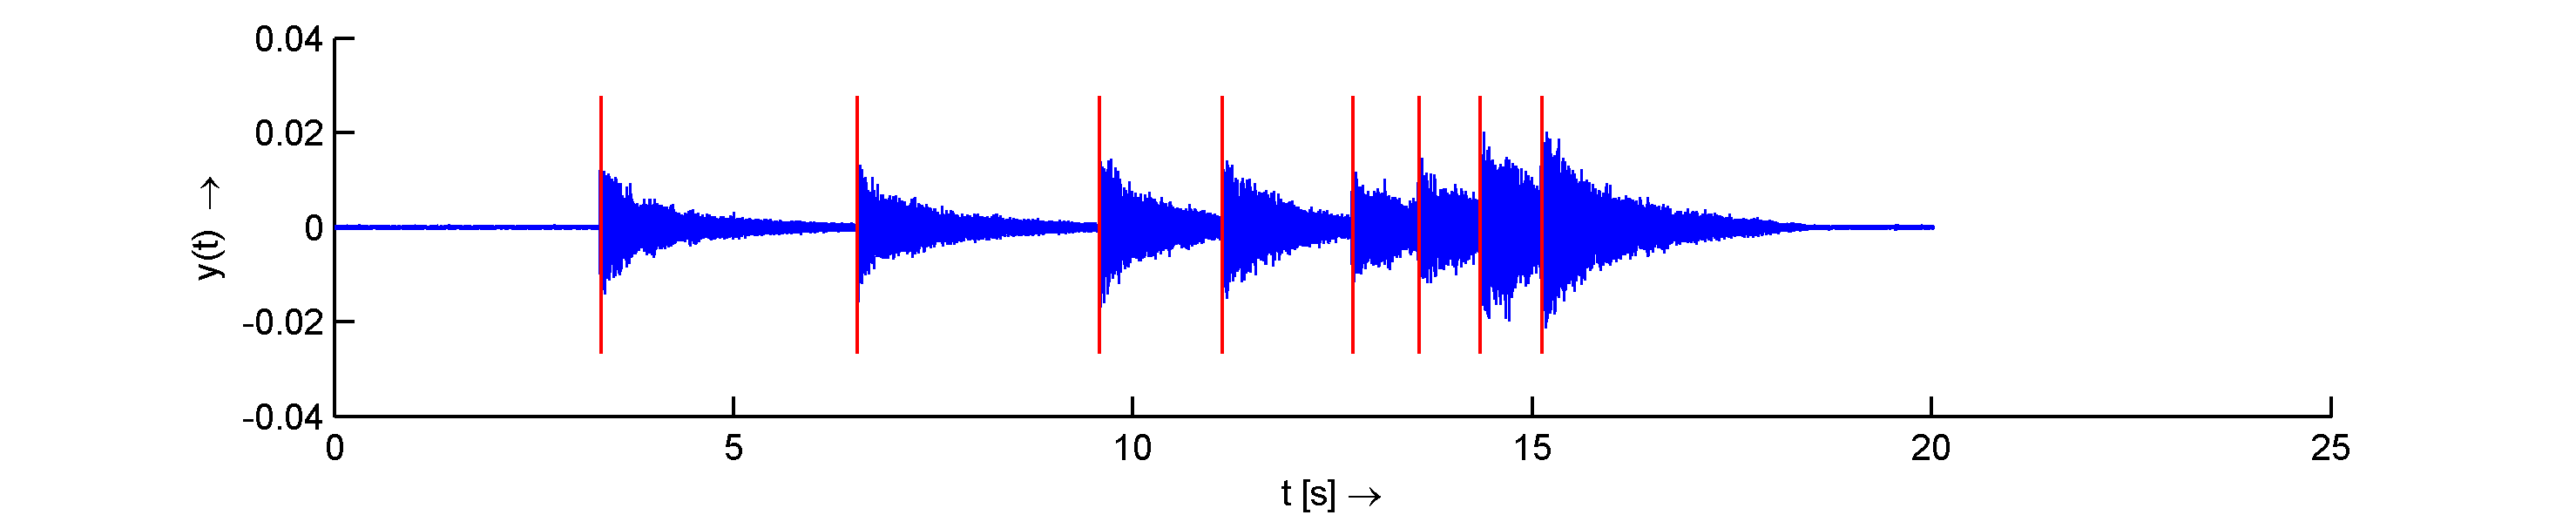
\includegraphics[width=7cm]{images/onsettest/1/drum_hihatopen.png}
	}
	\qquad
	\subfloat[Crash cymbal]{
		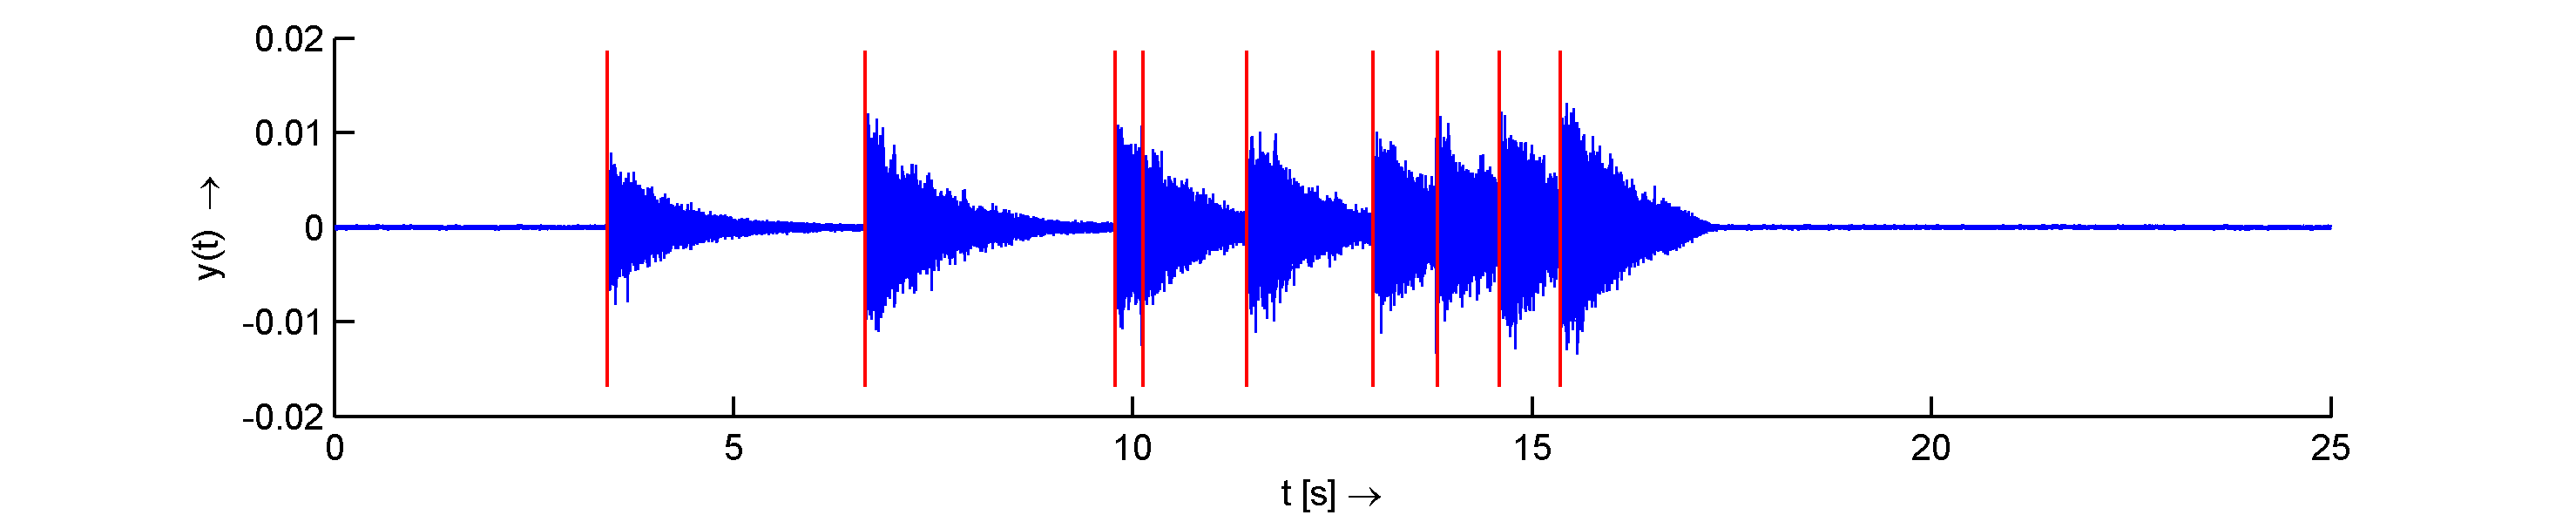
\includegraphics[width=7cm]{images/onsettest/1/drum_crash.png}
	 \label{fig:onsetTest1_1}
	}
	\subfloat[Ride cymbal]{
		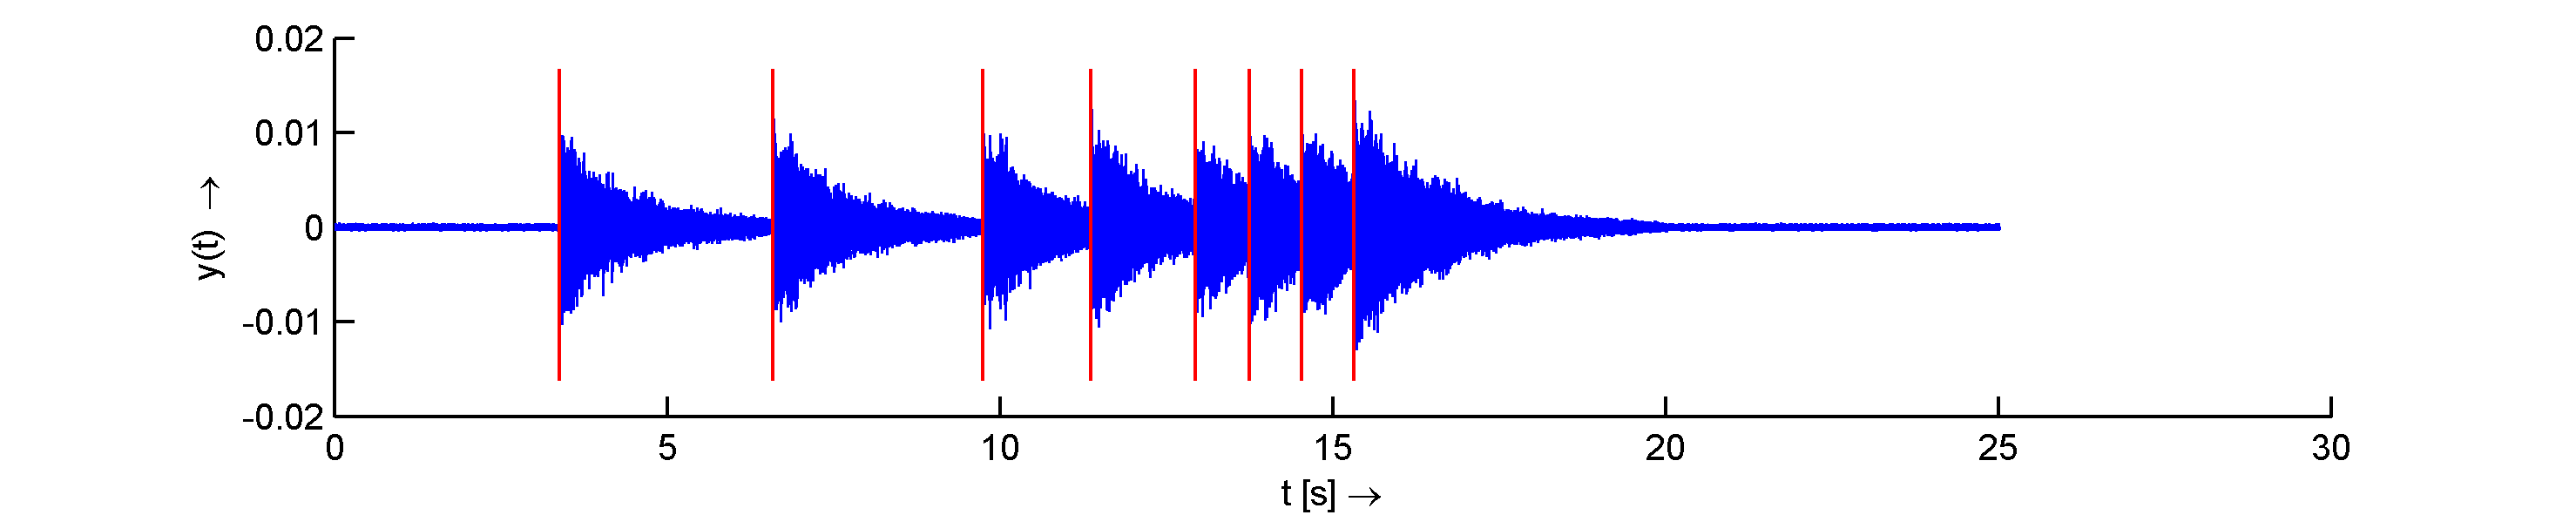
\includegraphics[width=7cm]{images/onsettest/1/drum_ride.png}
	}
	\qquad
	\subfloat[Loop 1]{
		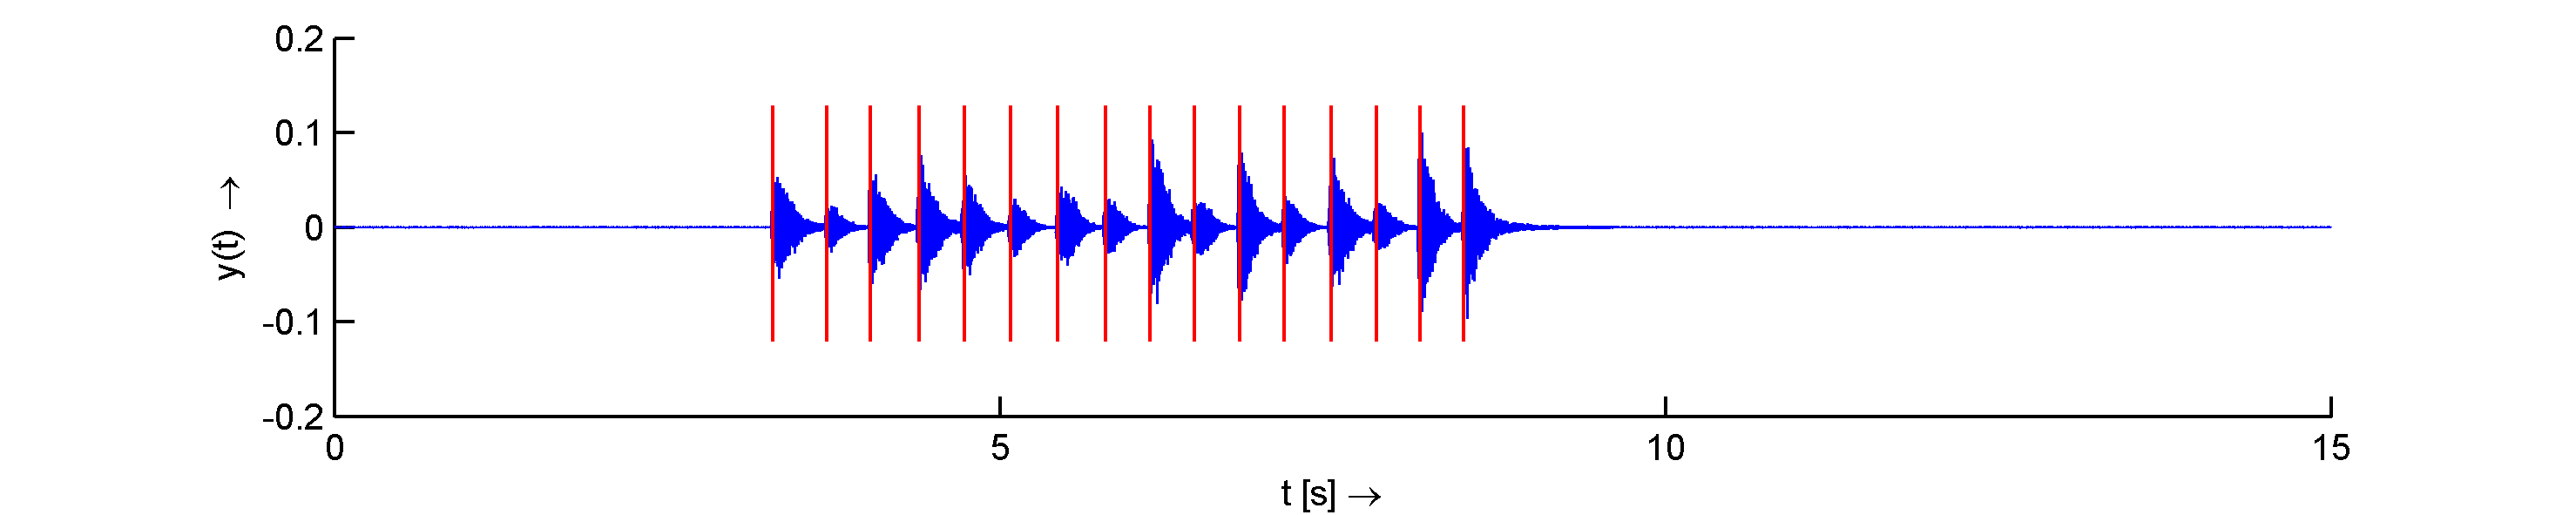
\includegraphics[width=7cm]{images/onsettest/1/loop1.png}
	}
	\subfloat[Loop 2]{
		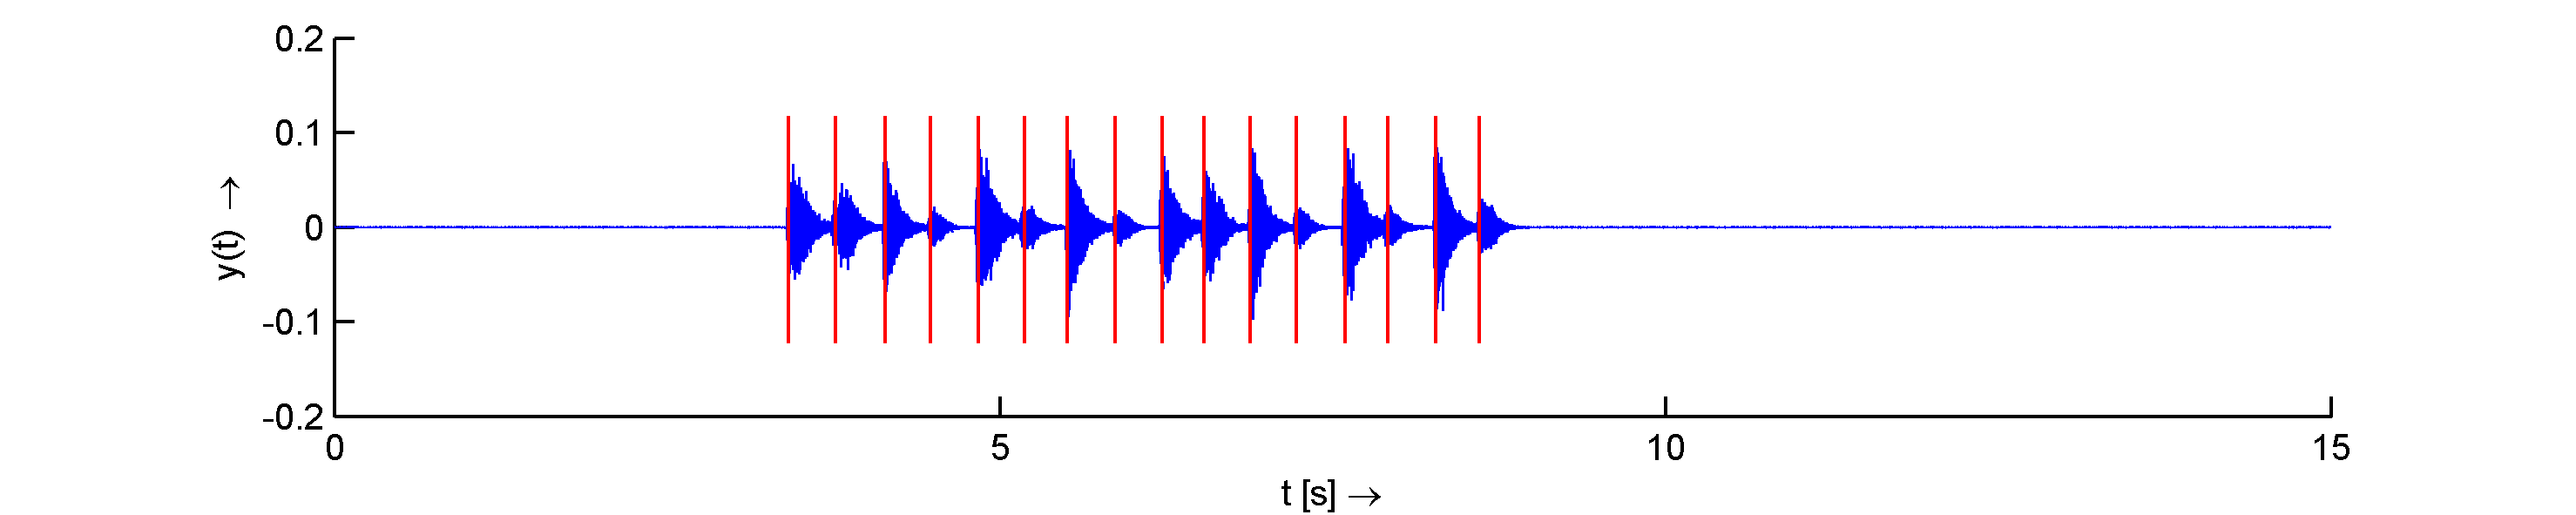
\includegraphics[width=7cm]{images/onsettest/1/loop2.png}
	}
	\qquad
	\subfloat[Loop 3]{
		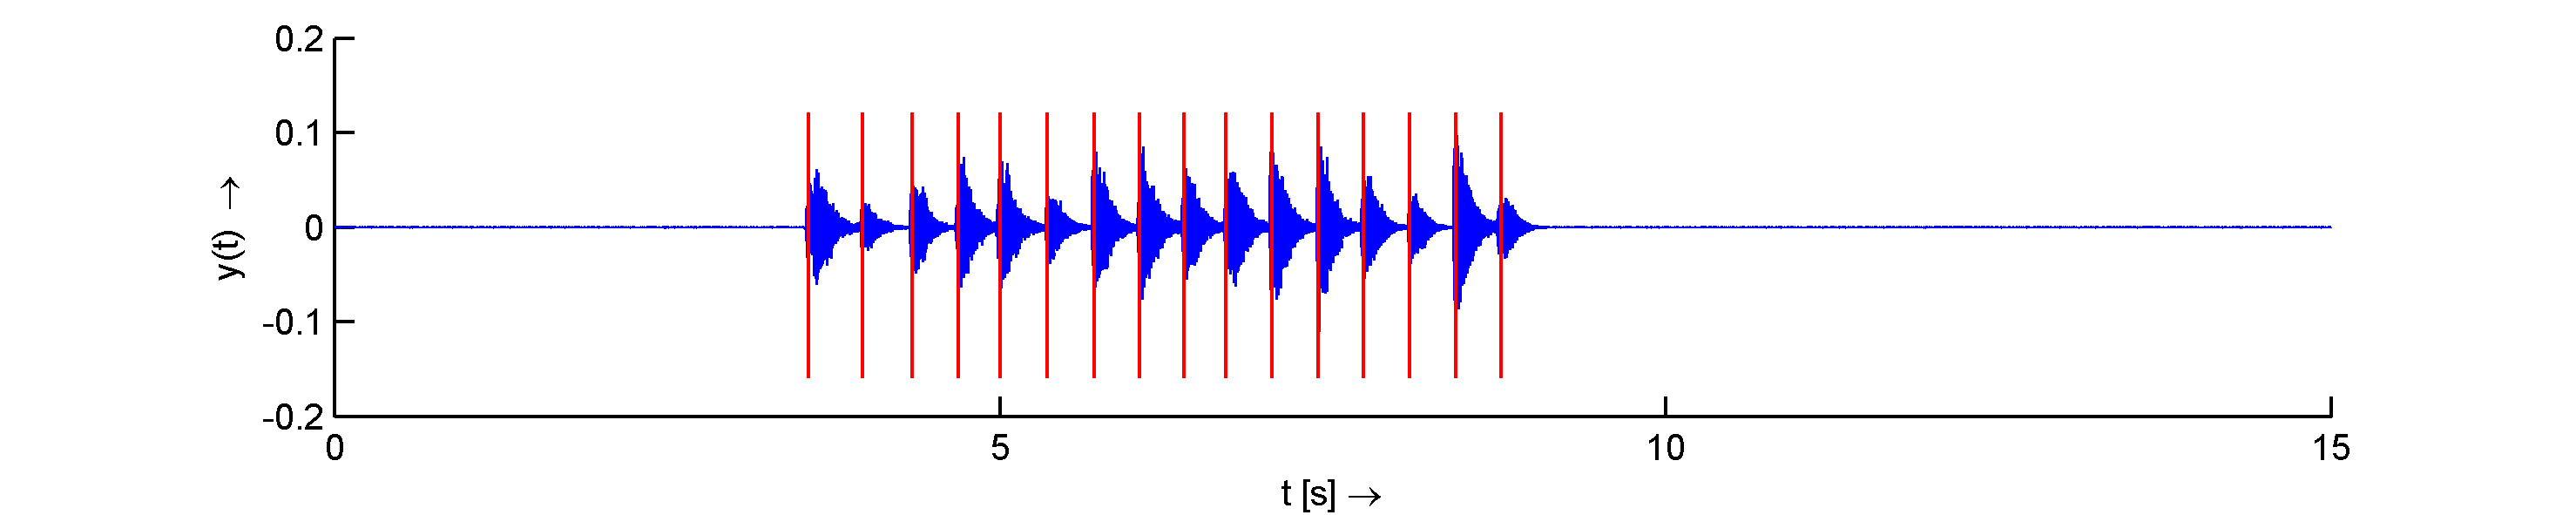
\includegraphics[width=7cm]{images/onsettest/1/loop3.png}
	}
	\subfloat[Loop 4]{
		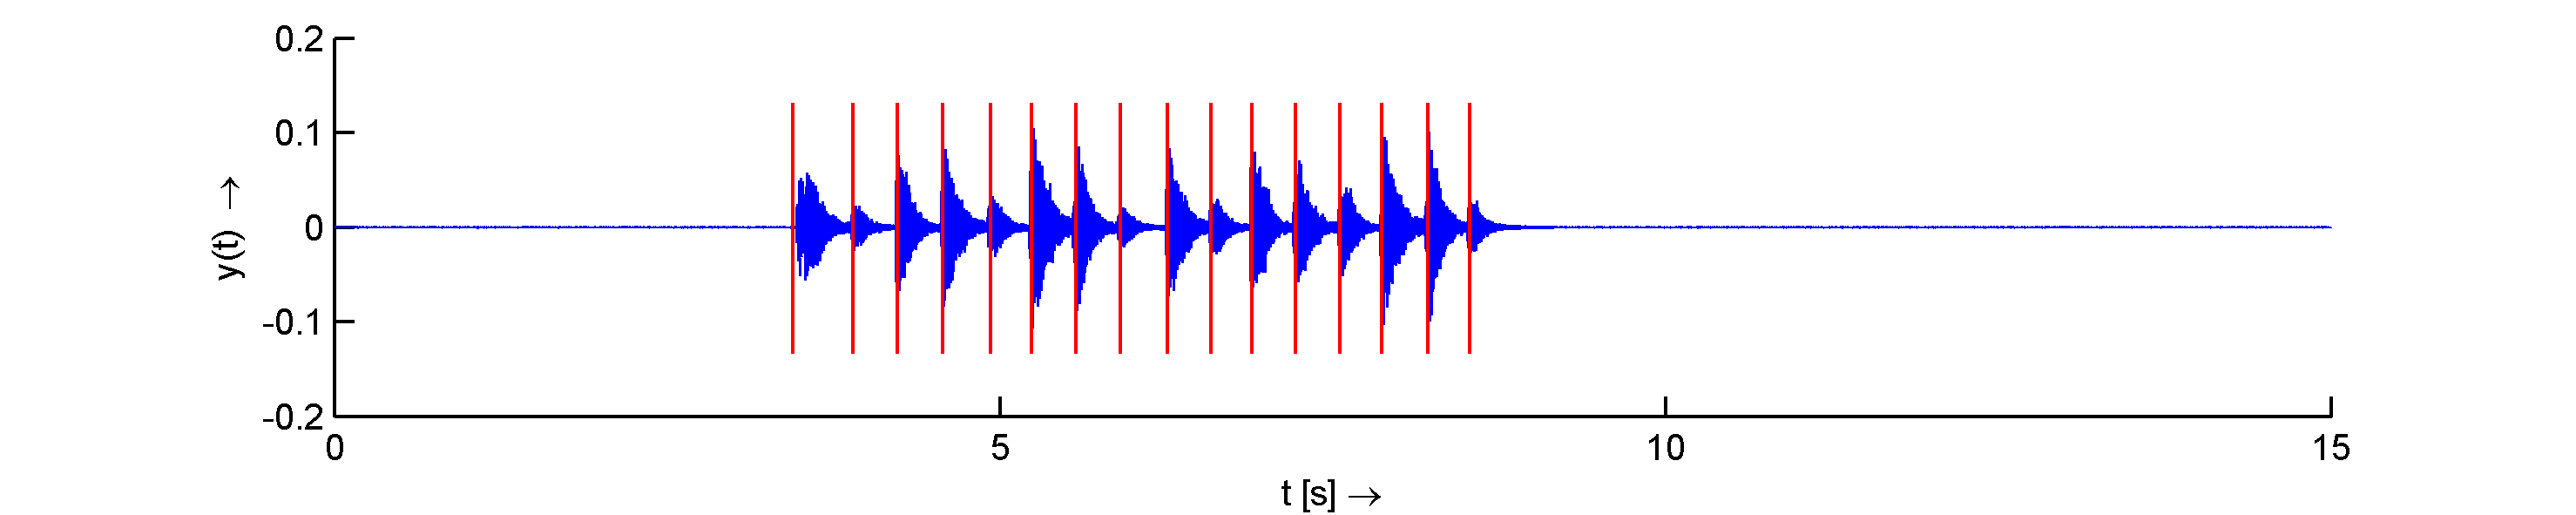
\includegraphics[width=7cm]{images/onsettest/1/loop4.png}
	}
	\qquad
	\subfloat[Fill-in 1 - snare drum, tom 1, tom 2, tom 3]{
		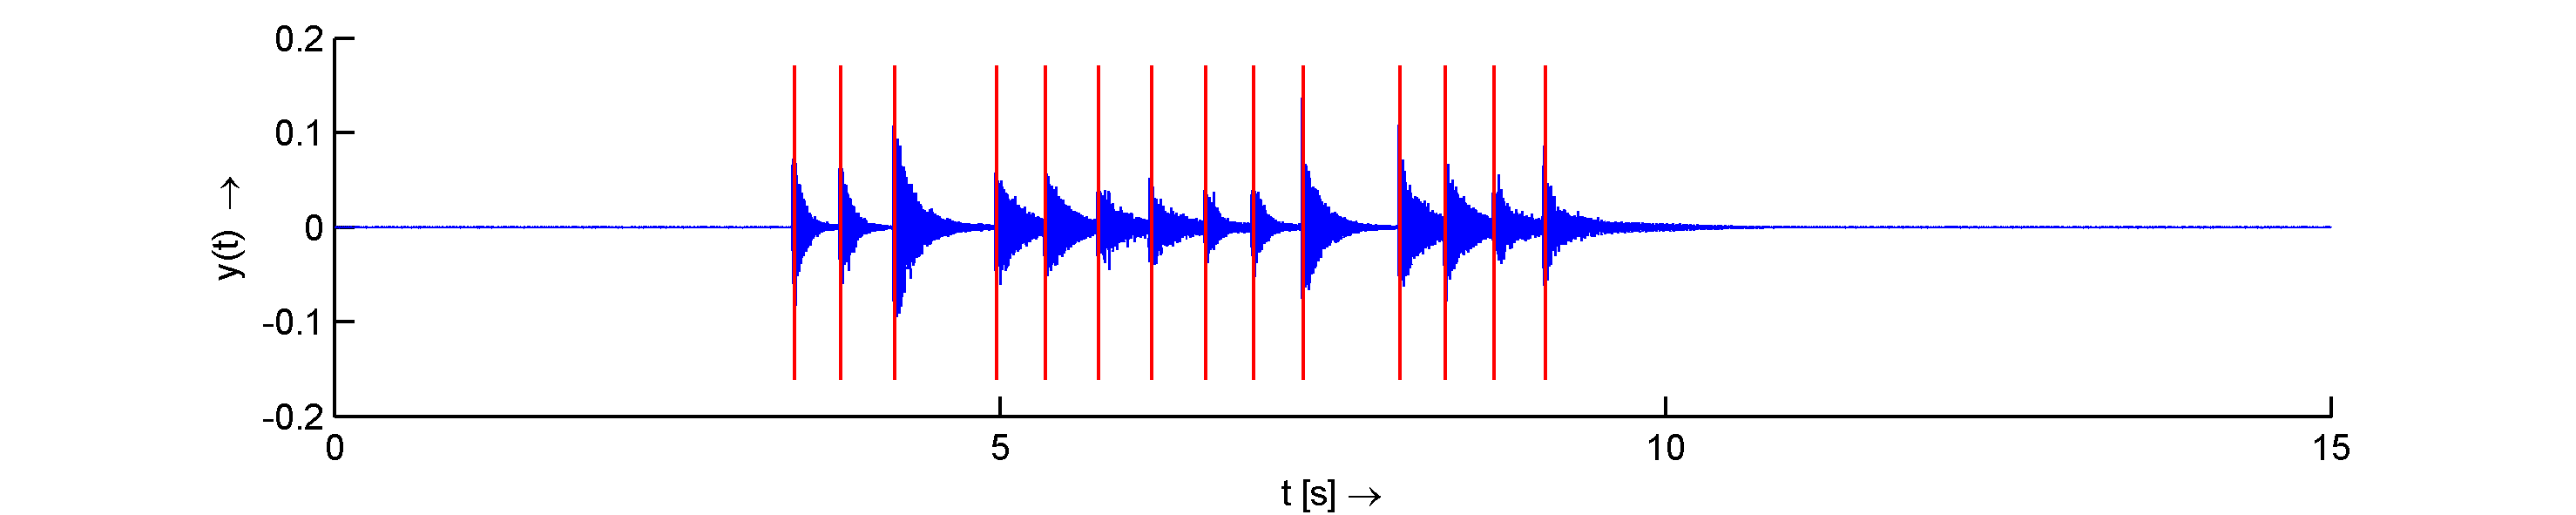
\includegraphics[width=7cm]{images/onsettest/1/fillin1.png}
	}
	\subfloat[Fill-in 2 - bass drum, snare drum, crash cymbal]{
		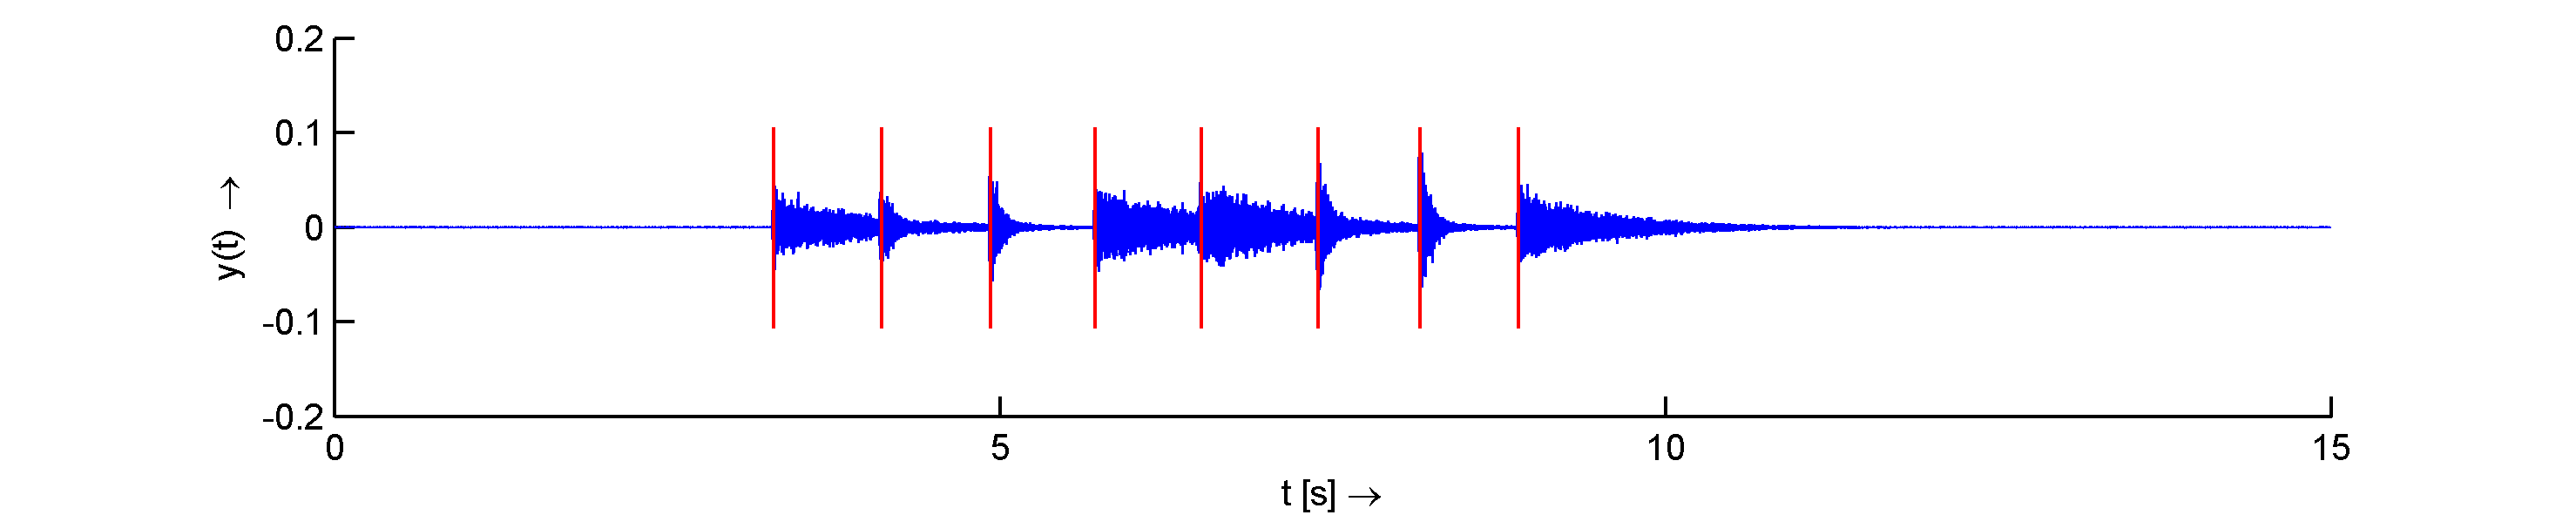
\includegraphics[width=7cm]{images/onsettest/1/fillin2.png}
	}
	\qquad
	\subfloat[Fill-in 3 - bass drum, snare drum, crash cymbal]{
		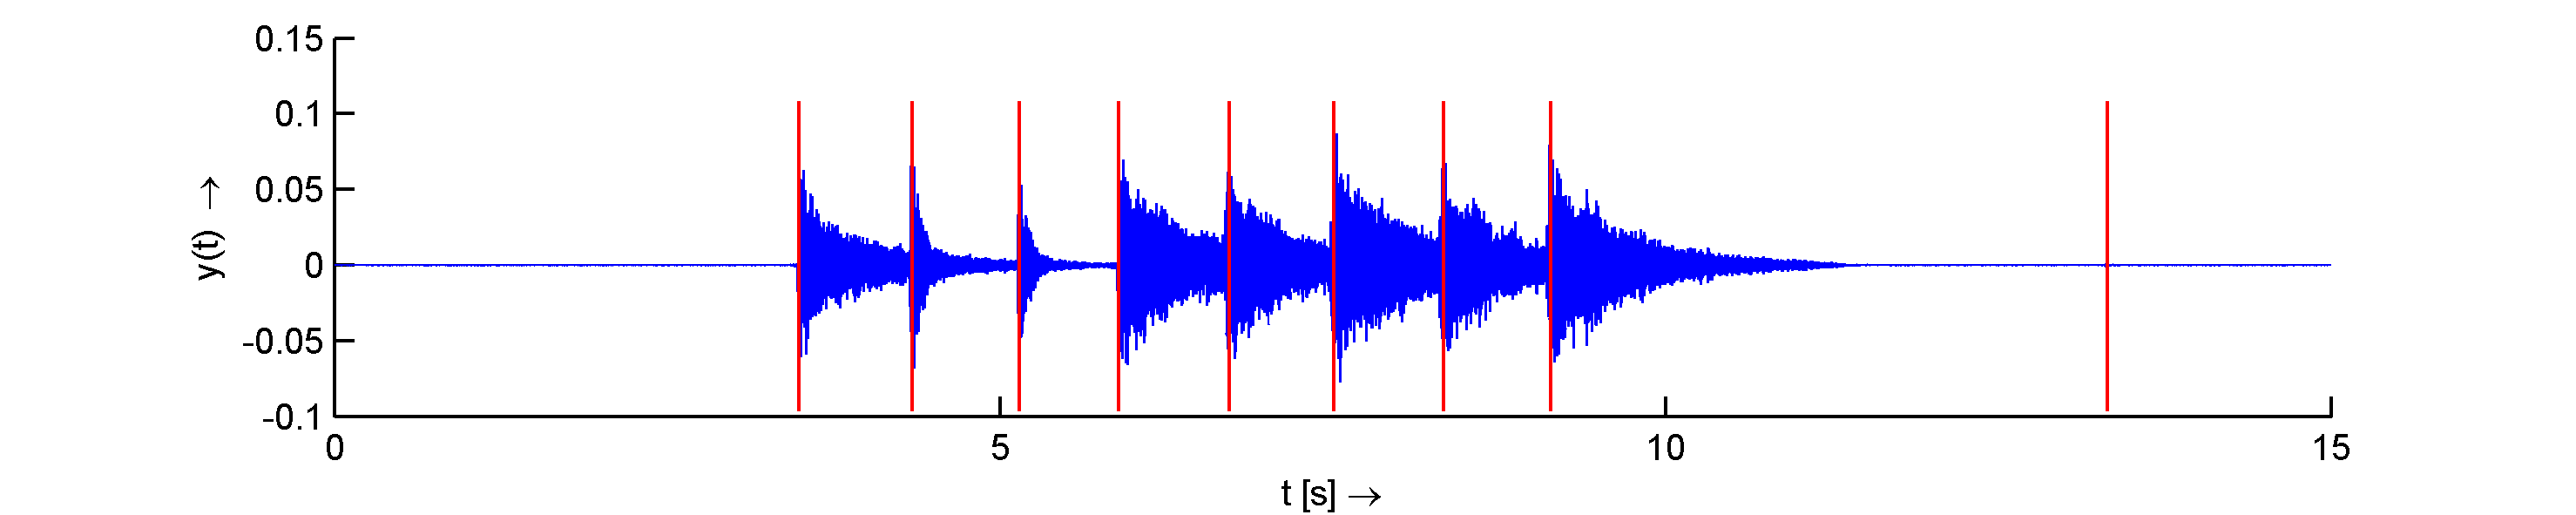
\includegraphics[width=7cm]{images/onsettest/1/fillin3.png}
	}
	\subfloat[Fill-in 4 - ride cymbal bow and bell]{
		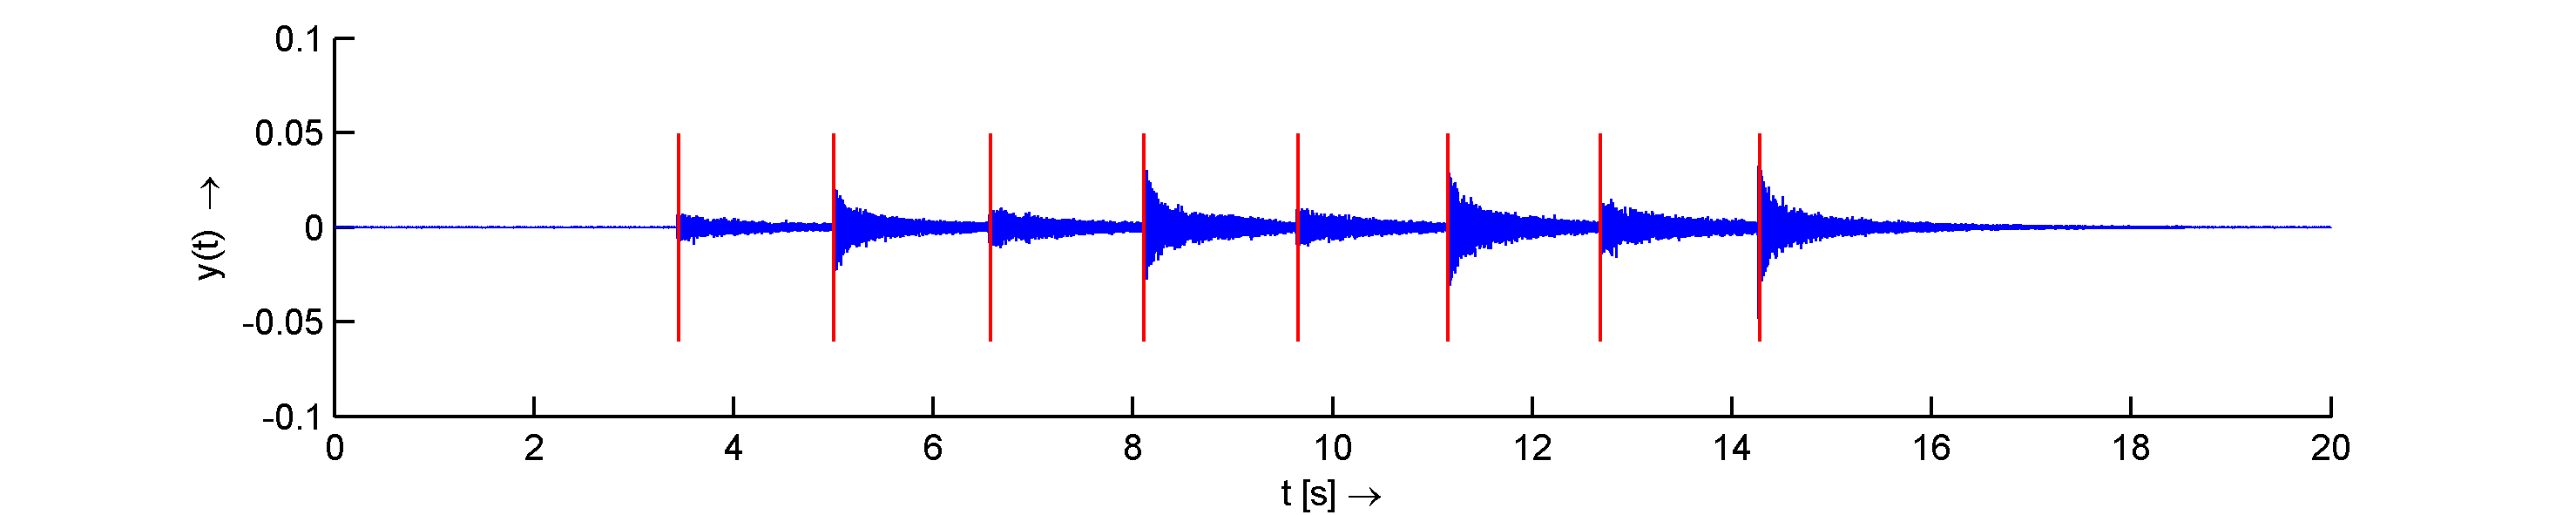
\includegraphics[width=7cm]{images/onsettest/1/fillin4.png}
	}
	\caption{Onset detection test 1.}
	\label{fig:onsetTest1}
\end{figure}


\begin{figure}[bp]
	\centering
	\subfloat[Bass drum]{
		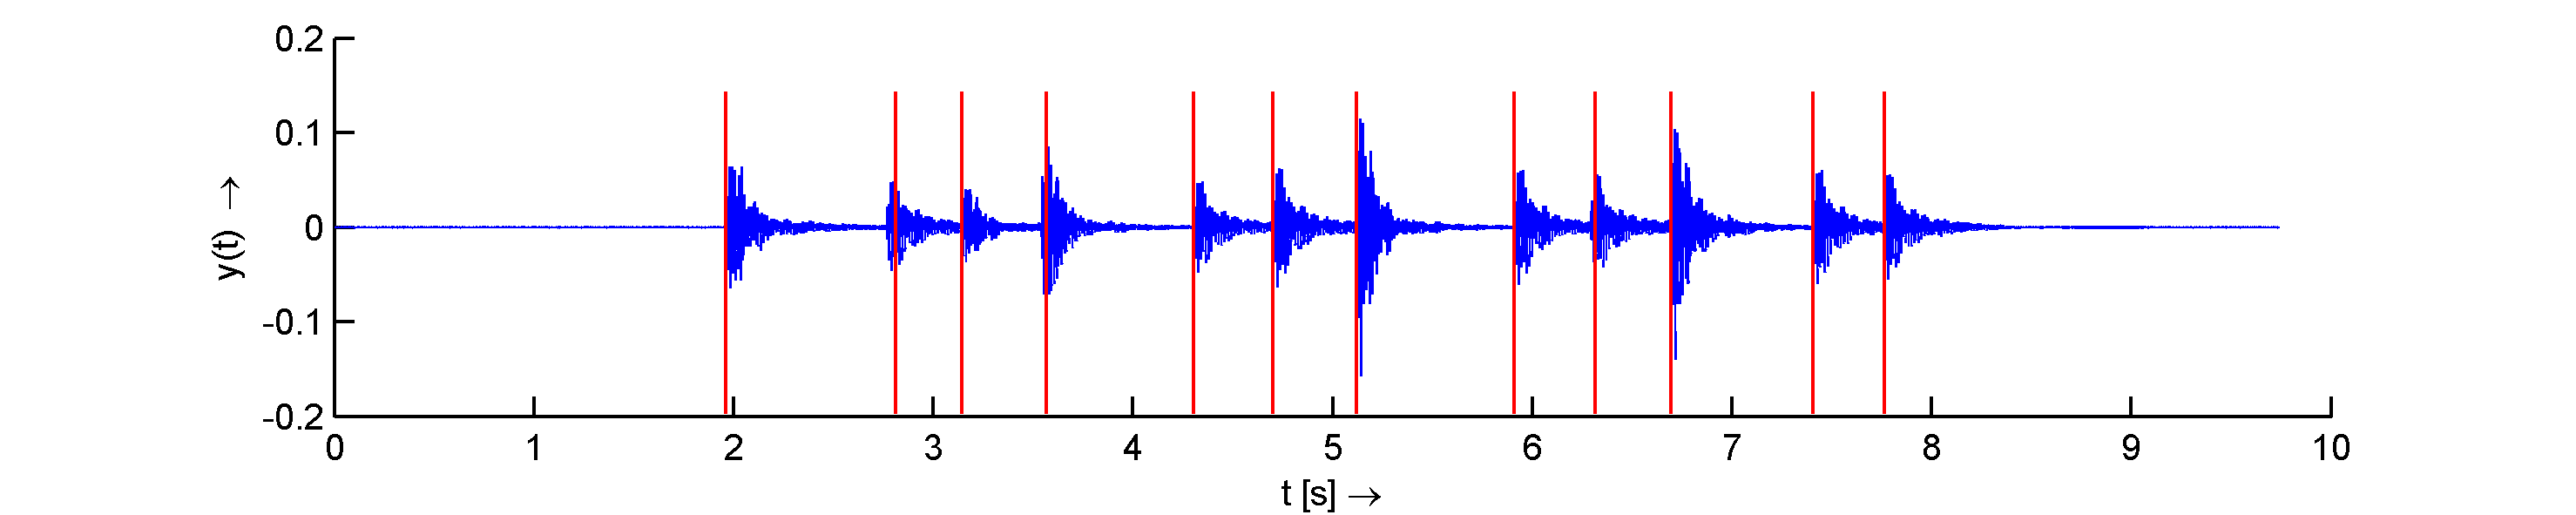
\includegraphics[width=7cm]{images/onsettest/2/drum_bass.png}
	}
	\subfloat[Snare drum 1]{
		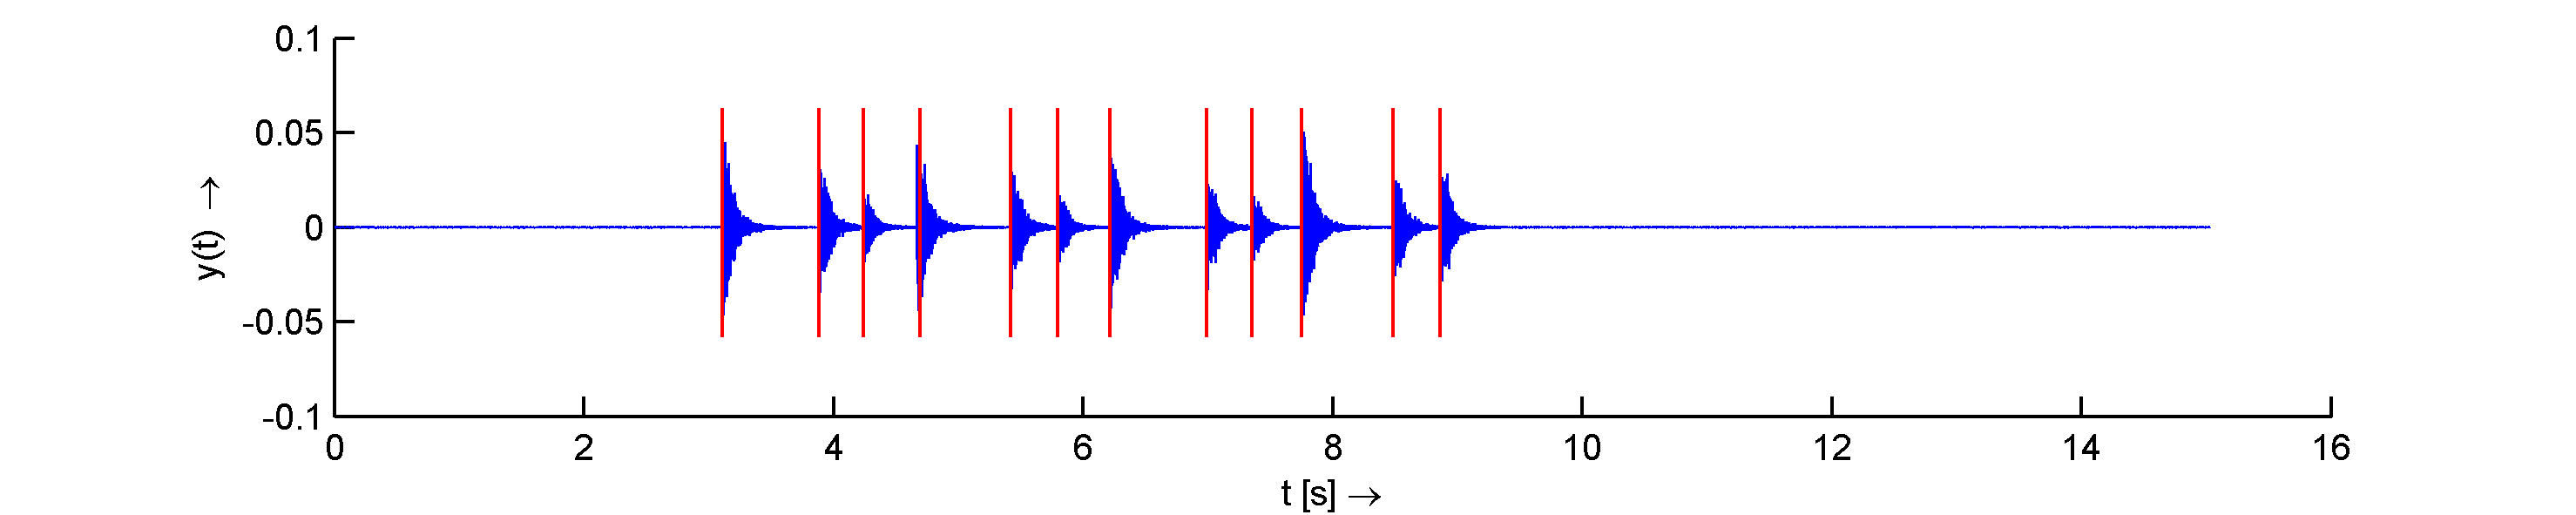
\includegraphics[width=7cm]{images/onsettest/2/drum_snare.png}
	}
	\qquad
	\subfloat[Snare drum 2]{
		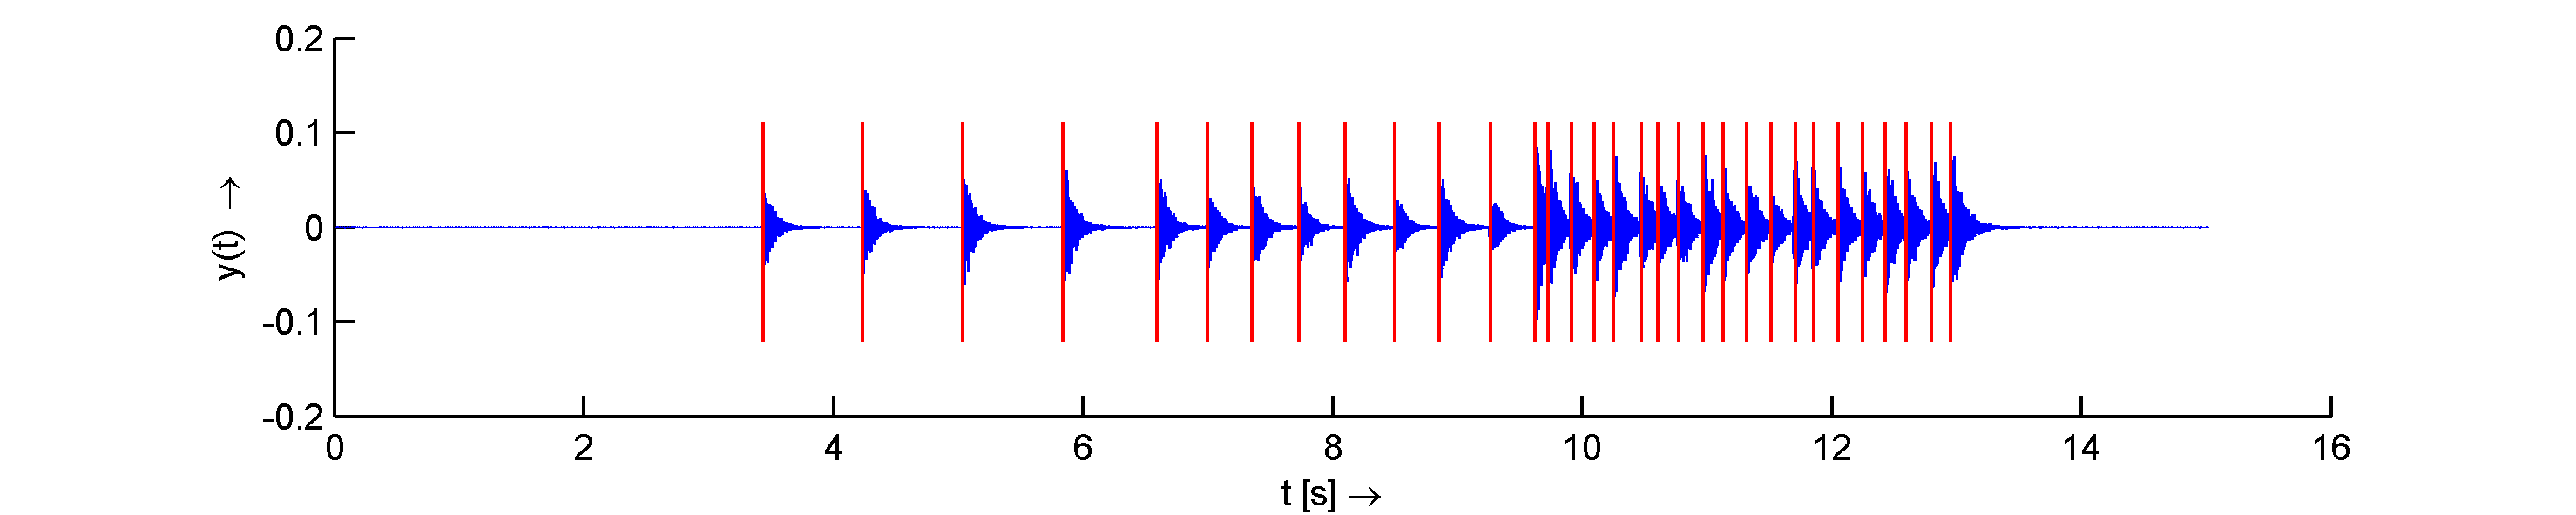
\includegraphics[width=7cm]{images/onsettest/2/drum_snare2.png}
	}
	\subfloat[Tom 1]{
		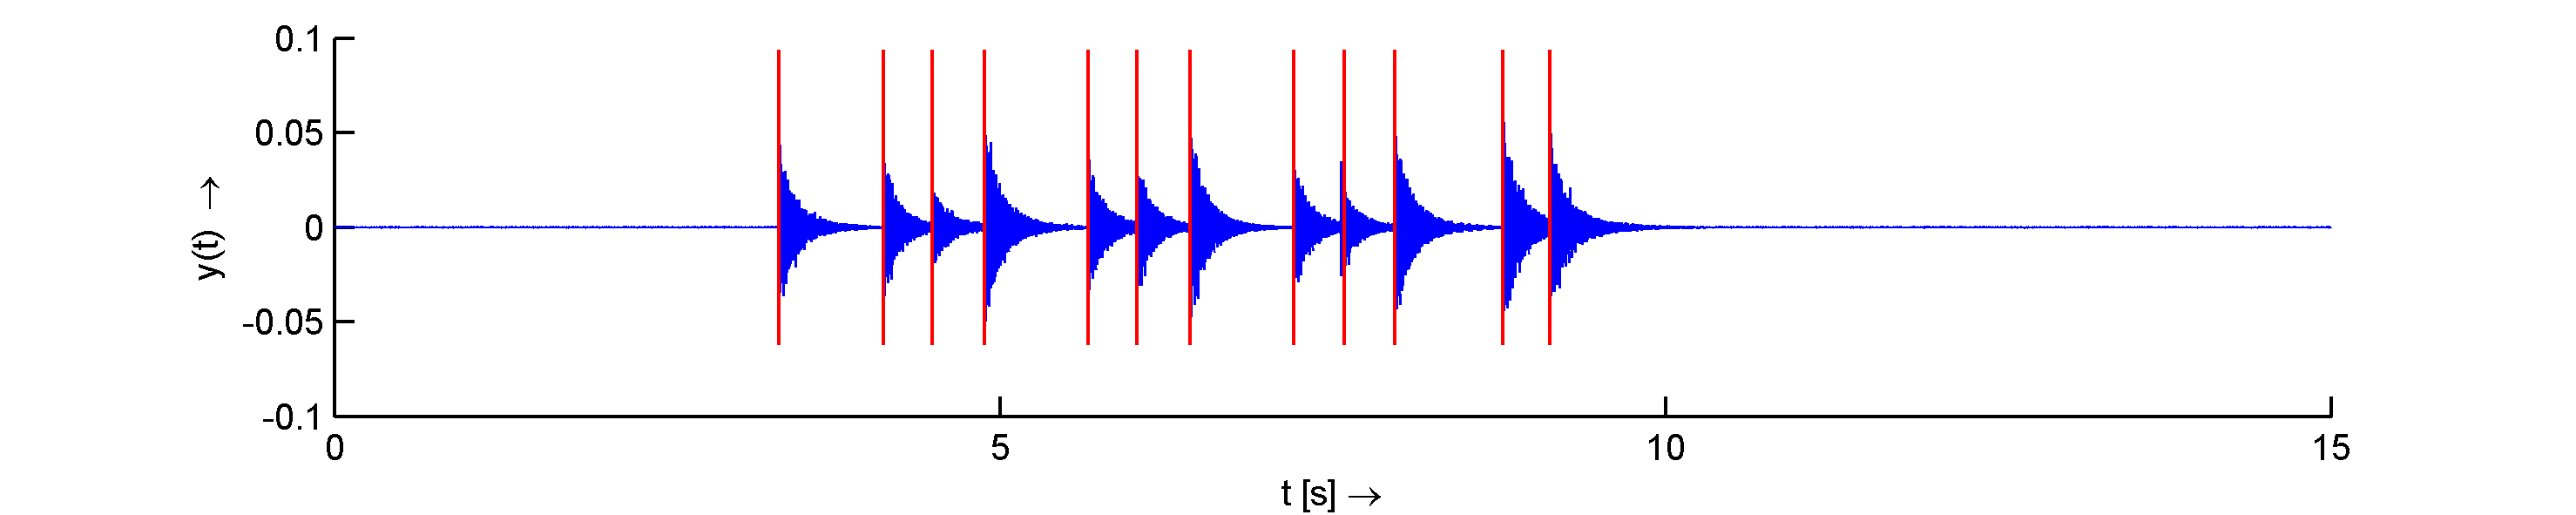
\includegraphics[width=7cm]{images/onsettest/2/drum_tom1.png}
	}
	\qquad
	\subfloat[Tom 2]{
		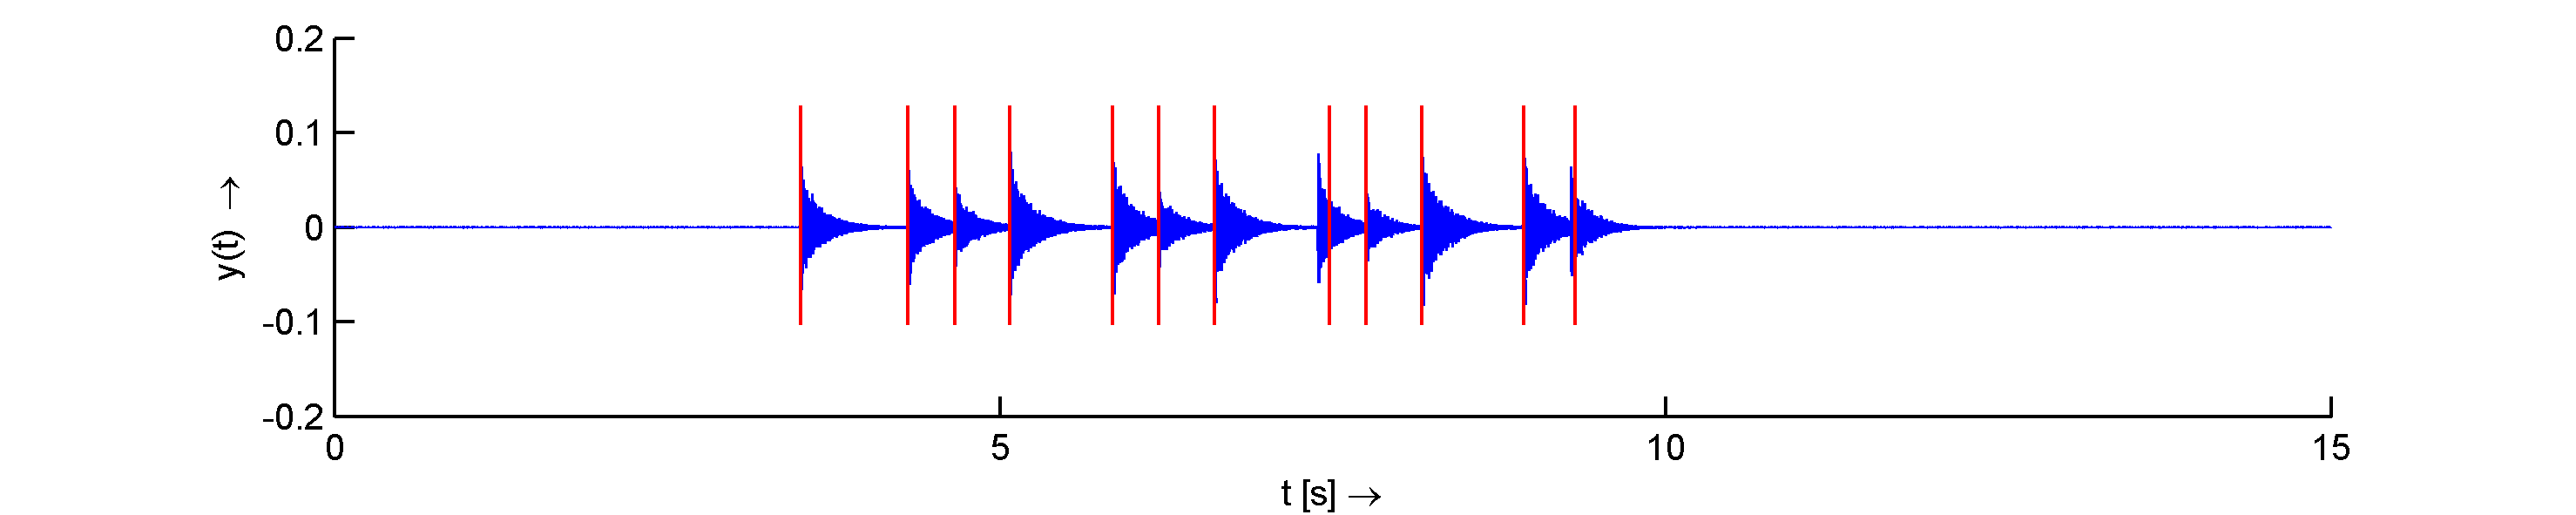
\includegraphics[width=7cm]{images/onsettest/2/drum_tom2.png}
	}
	\subfloat[Tom 3]{
		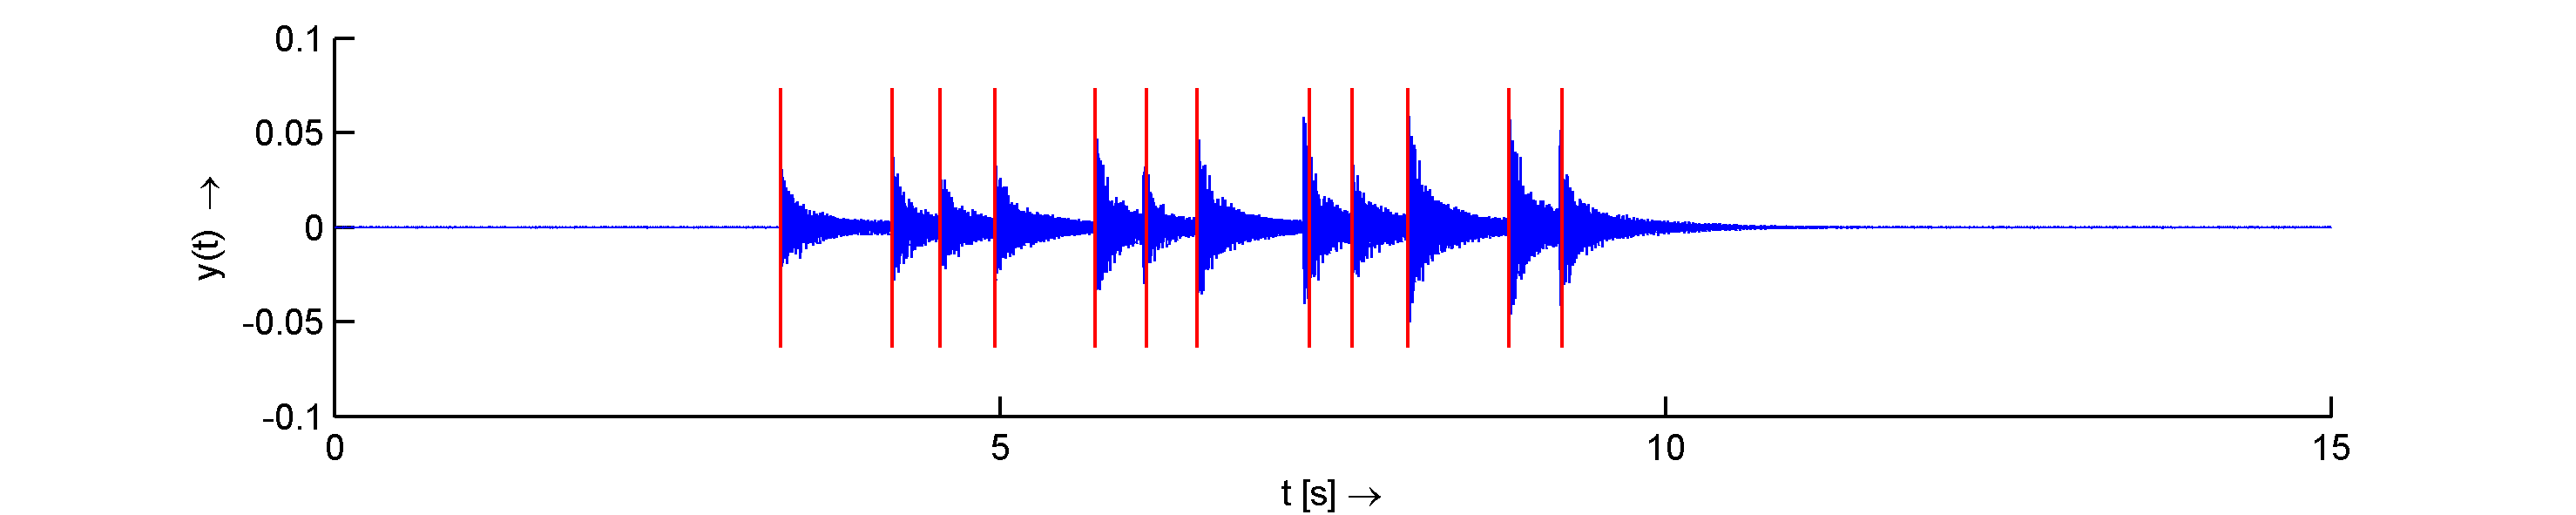
\includegraphics[width=7cm]{images/onsettest/2/drum_tom3.png}
	}
	\qquad
	\subfloat[Hi-hat closed]{
		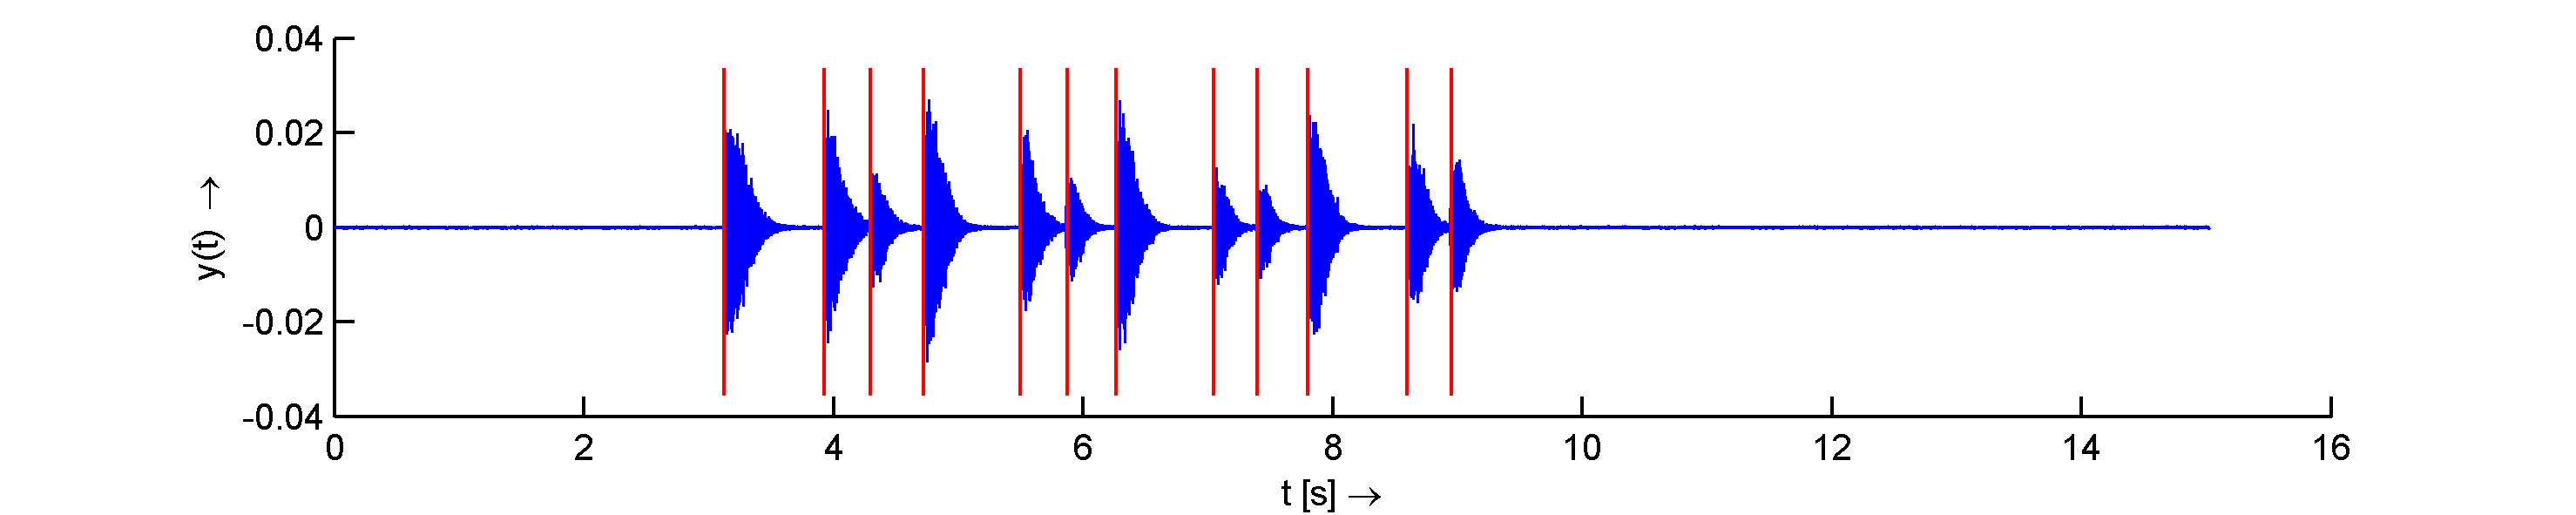
\includegraphics[width=7cm]{images/onsettest/2/drum_hihatclosed.png}
	}
	\subfloat[Hi-hat open]{
		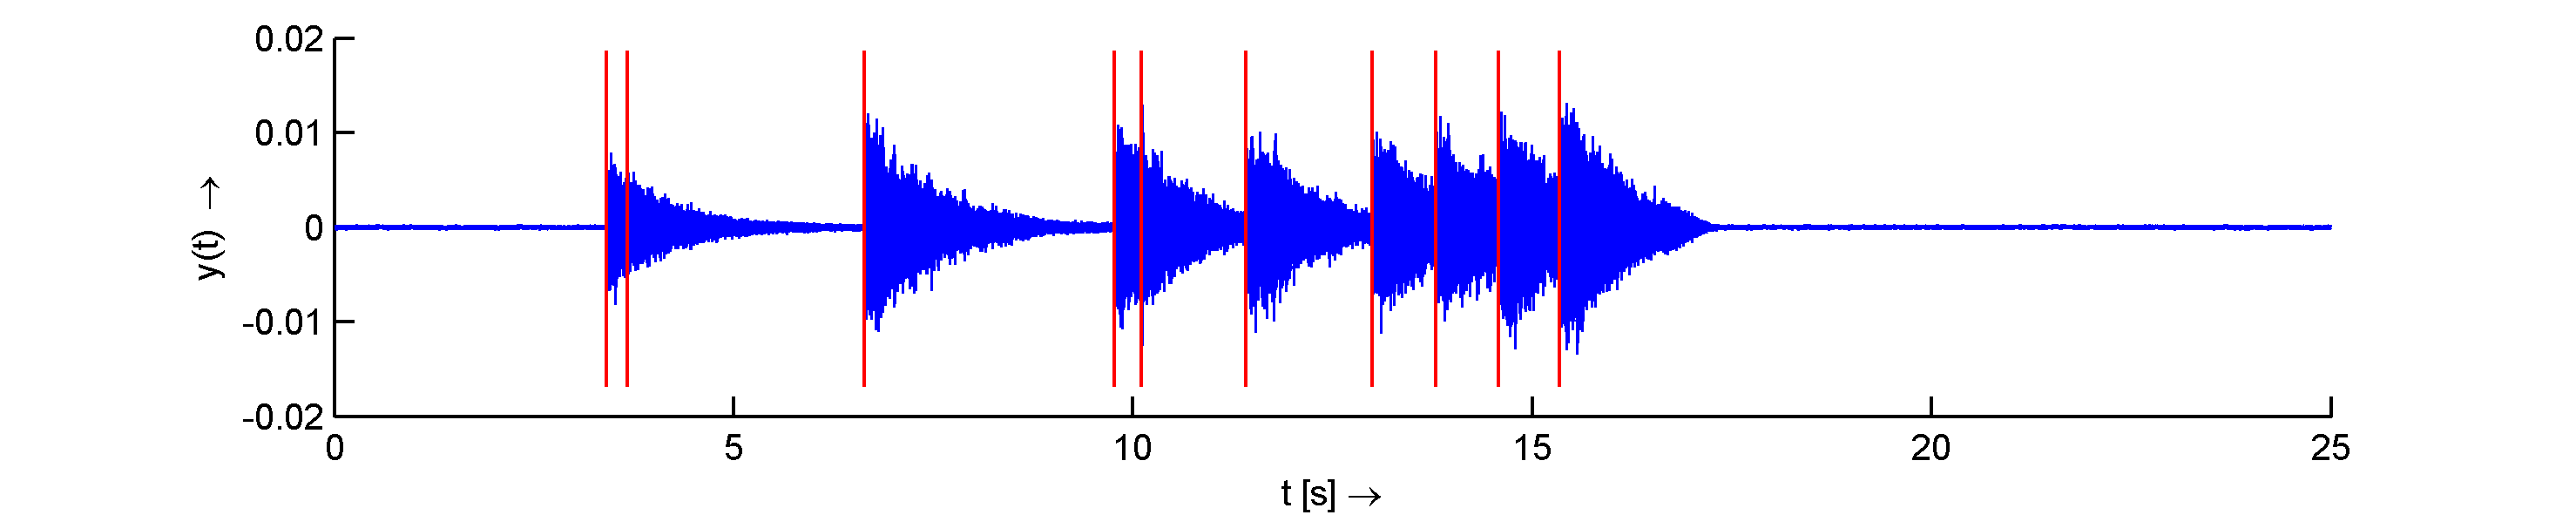
\includegraphics[width=7cm]{images/onsettest/2/drum_hihatopen.png}
	}
	\qquad
	\subfloat[Crash cymbal]{
		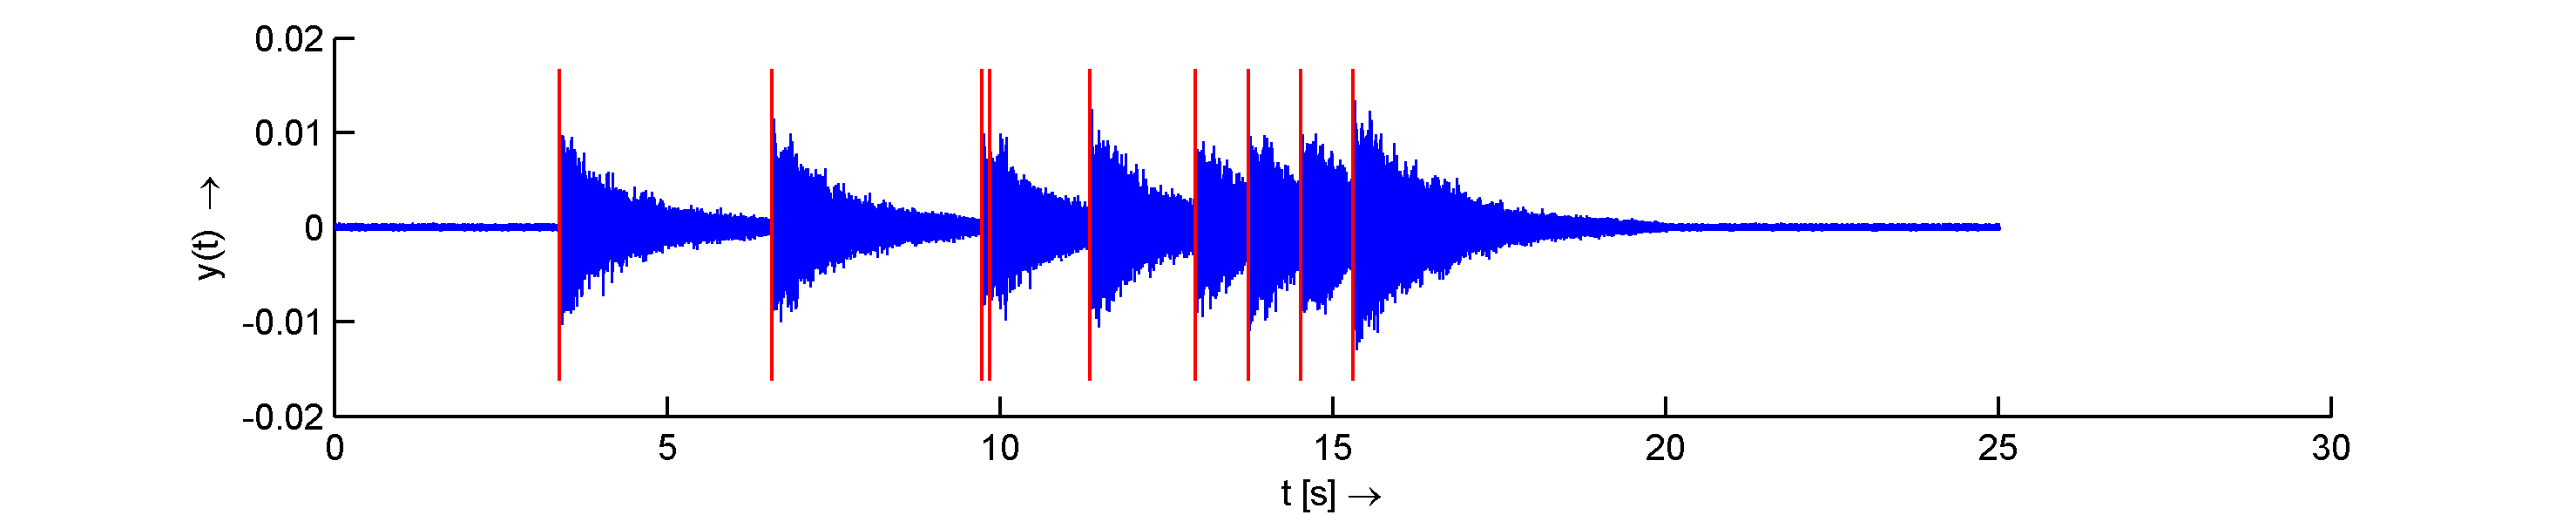
\includegraphics[width=7cm]{images/onsettest/2/drum_crash.png}
	}
	\subfloat[Ride cymbal]{
		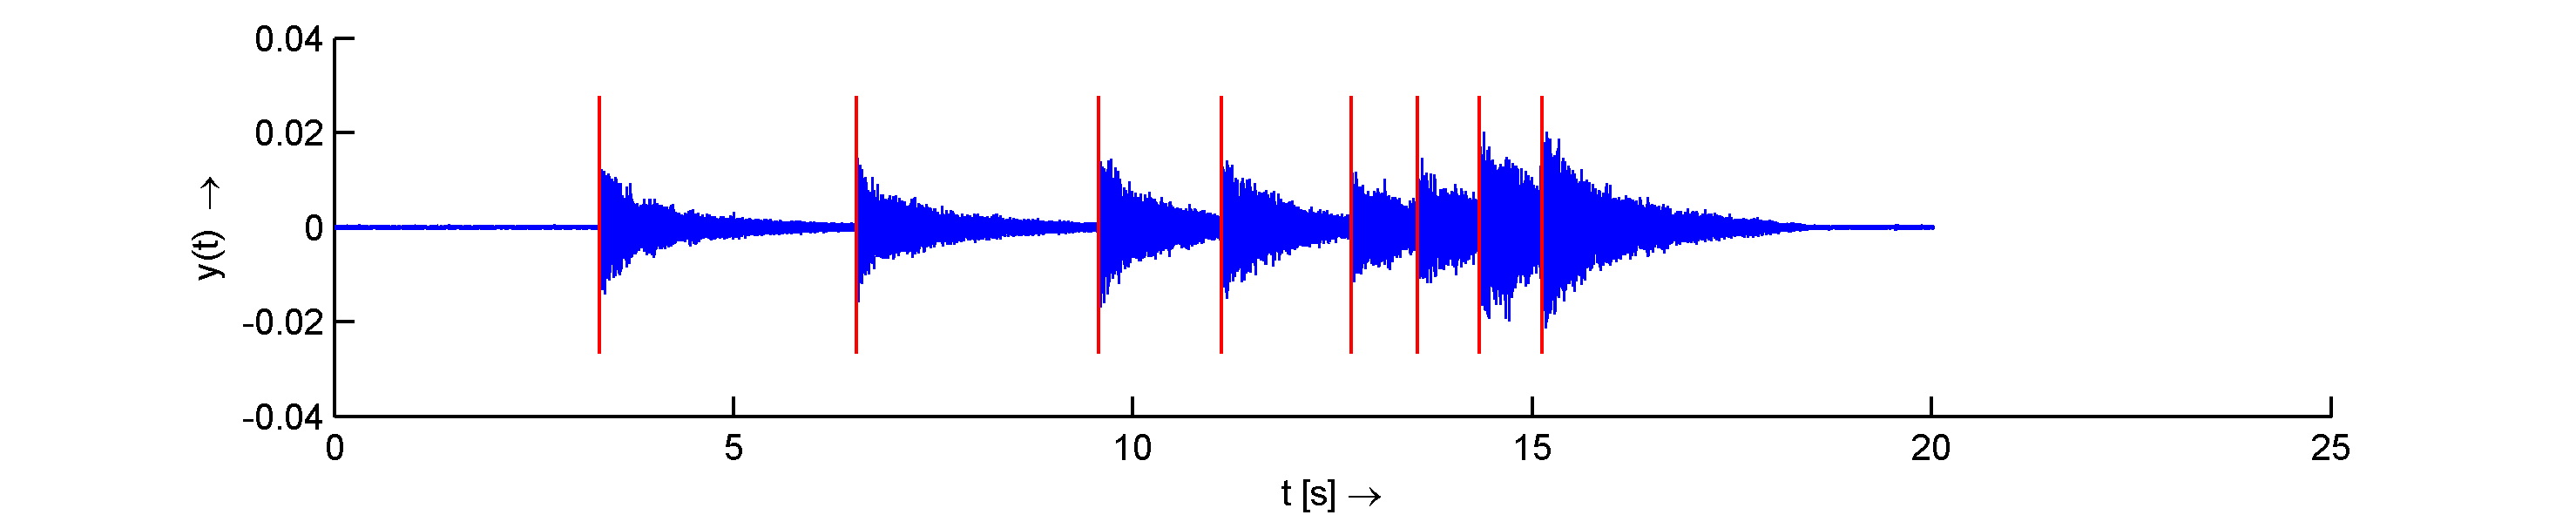
\includegraphics[width=7cm]{images/onsettest/2/drum_ride.png}
	}
	\qquad
	\subfloat[Loop 1]{
		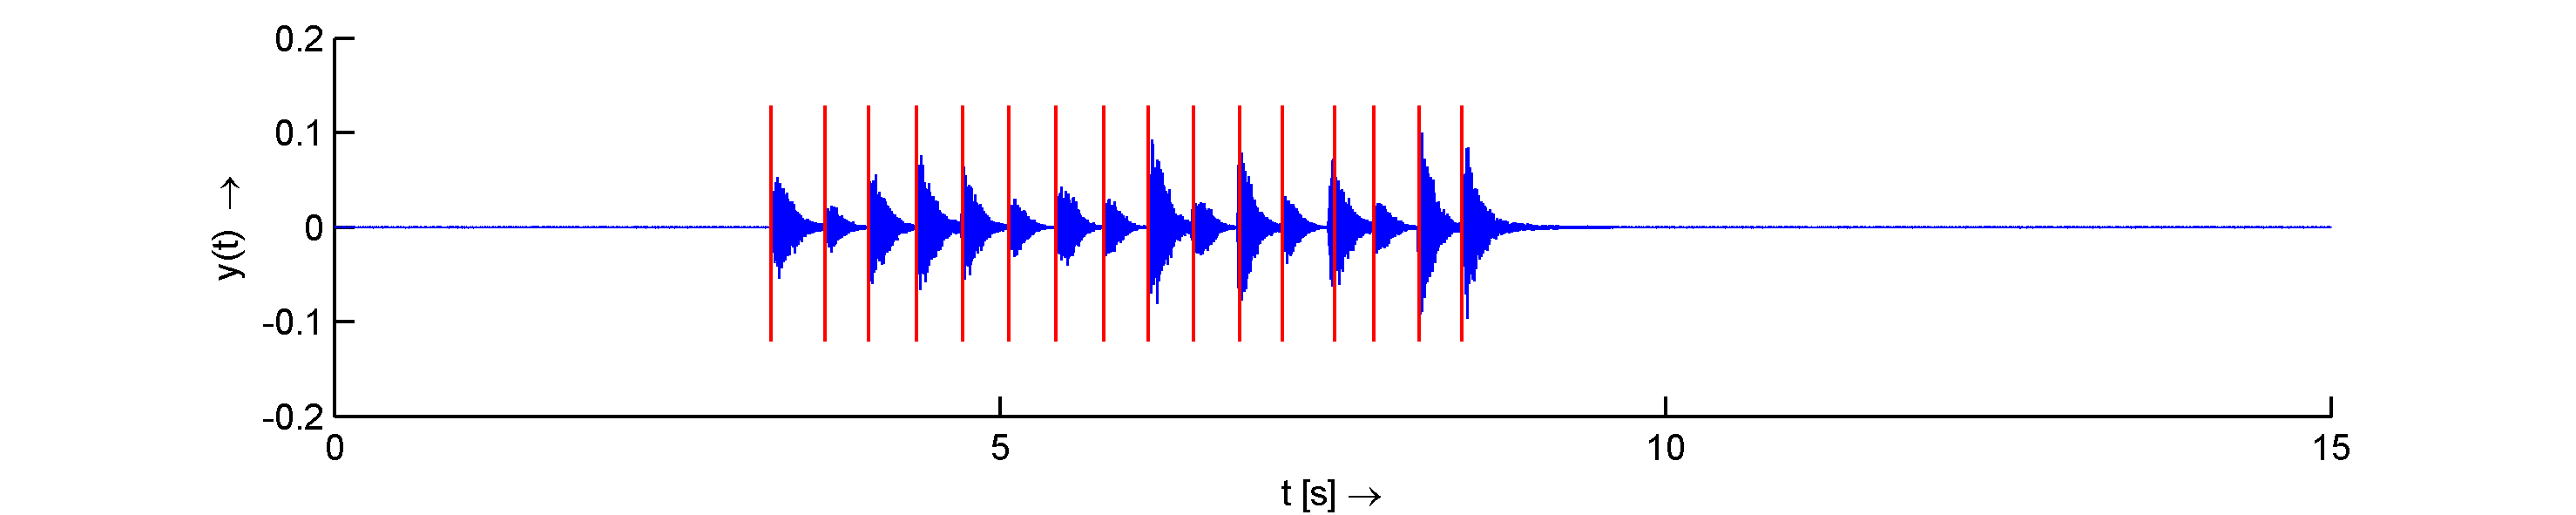
\includegraphics[width=7cm]{images/onsettest/2/loop1.png}
	}
	\subfloat[Loop 2]{
		\includegraphics[width=7cm]{images/onsettest/2/loop2.png}
	}
	\qquad
	\subfloat[Loop 3]{
		\includegraphics[width=7cm]{images/onsettest/2/loop3.png}
	}
	\subfloat[Loop 4]{
		\includegraphics[width=7cm]{images/onsettest/2/loop4.png}
	}
	\qquad
	\subfloat[Fill-in 1 - snare drum, tom 1, tom 2, tom 3]{
		\includegraphics[width=7cm]{images/onsettest/2/fillin1.png}
	}
	\subfloat[Fill-in 2 - bass drum, snare drum, crash cymbal]{
		\includegraphics[width=7cm]{images/onsettest/2/fillin2.png}
	}
	\qquad
	\subfloat[Fill-in 3 - bass drum, snare drum, crash cymbal]{
		\includegraphics[width=7cm]{images/onsettest/2/fillin3.png}
	}
	\subfloat[Fill-in 4 - ride cymbal bow and bell]{
		\includegraphics[width=7cm]{images/onsettest/2/fillin4.png}
	}
	\caption{Onset detection test 2.}
	\label{fig:onsetTest2}
\end{figure}


\begin{figure}[bp]
	\centering
	\subfloat[Bass drum]{
		\includegraphics[width=7cm]{images/onsettest/3/drum_bass.png}
	}
	\subfloat[Snare drum 1]{
		\includegraphics[width=7cm]{images/onsettest/3/drum_snare.png}
	}
	\qquad
	\subfloat[Snare drum 2]{
		\includegraphics[width=7cm]{images/onsettest/3/drum_snare2.png}
	}
	\subfloat[Tom 1]{
		\includegraphics[width=7cm]{images/onsettest/3/drum_tom1.png}
	}
	\qquad
	\subfloat[Tom 2]{
		\includegraphics[width=7cm]{images/onsettest/3/drum_tom2.png}
	}
	\subfloat[Tom 3]{
		\includegraphics[width=7cm]{images/onsettest/3/drum_tom3.png}
	}
	\qquad
	\subfloat[Hi-hat closed]{
		\includegraphics[width=7cm]{images/onsettest/3/drum_hihatclosed.png}
	}
	\subfloat[Hi-hat open]{
		\includegraphics[width=7cm]{images/onsettest/3/drum_hihatopen.png}
	}
	\qquad
	\subfloat[Crash cymbal]{
		\includegraphics[width=7cm]{images/onsettest/3/drum_crash.png}
	}
	\subfloat[Ride cymbal]{
		\includegraphics[width=7cm]{images/onsettest/3/drum_ride.png}
	}
	\qquad
	\subfloat[Loop 1]{
		\includegraphics[width=7cm]{images/onsettest/3/loop1.png}
	}
	\subfloat[Loop 2]{
		\includegraphics[width=7cm]{images/onsettest/3/loop2.png}
	}
	\qquad
	\subfloat[Loop 3]{
		\includegraphics[width=7cm]{images/onsettest/3/loop3.png}
	}
	\subfloat[Loop 4]{
		\includegraphics[width=7cm]{images/onsettest/3/loop4.png}
	}
	\qquad
	\subfloat[Fill-in 1 - snare drum, tom 1, tom 2, tom 3]{
		\includegraphics[width=7cm]{images/onsettest/3/fillin1.png}
	}
	\subfloat[Fill-in 2 - bass drum, snare drum, crash cymbal]{
		\includegraphics[width=7cm]{images/onsettest/3/fillin2.png}
	}
	\qquad
	\subfloat[Fill-in 3 - bass drum, snare drum, crash cymbal]{
		\includegraphics[width=7cm]{images/onsettest/3/fillin3.png}
	}
	\subfloat[Fill-in 4 - ride cymbal bow and bell]{
		\includegraphics[width=7cm]{images/onsettest/3/fillin4.png}
	}
	\caption{Onset detection test 3.}
	\label{fig:onsetTest3}
\end{figure}

